\documentclass[aspectratio=43]{beamer}

% Title --------------------------------------------
\title{\huge Rebel groups}
\author{Francisco Villamil}
\date{War, peace, and political violence\\UC3M, Fall 2023}

%%% NOTE -- CHECK THIS: https://github.com/paulgp/beamer-tips


%%% Building heavily on https://github.com/kylebutts/templates

% xcolor, define them
\usepackage{xcolor}

% TEXT COLORS
\definecolor{red}{HTML}{9a2515}
\definecolor{yellow}{HTML}{EBC944}
\definecolor{asher}{HTML}{555F61}
\definecolor{jet}{HTML}{131516}

% THEME COLORS
\definecolor{accent}{HTML}{107895}
\definecolor{accent2}{HTML}{9a2515}

% Color commands
\newcommand\red[1]{{\color{red}#1}}
\newcommand\yellow[1]{{\color{yellow}#1}}
\newcommand\asher[1]{{\color{asher}#1}}

\newcommand\BGred[1]{{\colorbox{red!80!white}{#1}}}
\newcommand\BGyellow[1]{{\colorbox{yellow!80!white}{#1}}}
\newcommand\BGasher[1]{{\colorbox{asher!80!white}{#1}}}

\renewcommand<>{\BGyellow}[1]{\only#2{\beameroriginal{\BGyellow}}{#1}}

% Appendix numbering
\usepackage{appendixnumberbeamer}

% Beamer Options -------------------------------------

% Background
\setbeamercolor{background canvas}{bg = white}

% Change text margins
\setbeamersize{text margin left = 25pt, text margin right = 15pt}

% \alert
\setbeamercolor{alerted text}{fg = accent2}

% Frame title
\setbeamercolor{frametitle}{bg = white, fg = jet}
\setbeamercolor{framesubtitle}{bg = white, fg = accent}
\setbeamerfont{framesubtitle}{size = \small, shape = \itshape}

% Block
\setbeamercolor{block title}{fg = white, bg = accent2}
\setbeamercolor{block body}{fg = jet, bg = jet!10!white}

% Title page
\setbeamercolor{title}{fg = jet}
\setbeamercolor{subtitle}{fg = accent}

%% Custom \maketitle and \titlepage
\setbeamertemplate{title page}
{
    \begin{centering}
      % \vspace{20mm}
      {\Large \usebeamerfont{title}\usebeamercolor[fg]{title}\inserttitle}\\ \vskip0.25em%
      \ifx\insertsubtitle\@empty%
      \else%
        {\usebeamerfont{subtitle}\usebeamercolor[fg]{subtitle}\insertsubtitle\par}%
      \fi%
      {\vspace{10mm}\insertauthor}\\
      \ifx\insertinstitute\@empty%
      \else%
        {\vspace{5mm}\color{asher}\scriptsize{\insertinstitute}}
      \fi%
      {\color{asher}\small{\insertdate}}\\
    \end{centering}
}

% Table of Contents
\setbeamercolor{section in toc}{fg = accent!70!jet}
\setbeamercolor{subsection in toc}{fg = jet}

% Button
\setbeamercolor{button}{bg = accent}

% Remove navigation symbols
\setbeamertemplate{navigation symbols}{}

% Table and Figure captions
\setbeamercolor{caption}{fg=jet!70!white}
\setbeamercolor{caption name}{fg=jet}
\setbeamerfont{caption name}{shape = \itshape}

% Put slide number / total slides at the bottom right
\makeatother
\makeatletter
\setbeamertemplate{footline} %{\hfill\insertframenumber/\inserttotalframenumber}
{%
  \leavevmode%
  \hbox{
  \begin{beamercolorbox}[wd=\paperwidth,ht=2.5ex,dp=1.125ex,leftskip=.3cm,rightskip=.3cm plus1fil]{footlinecolor}%
    \color{asher}{\hfill\insertframenumber/\inserttotalframenumber}
  \end{beamercolorbox}}%
  \vskip0pt%
}
\makeatother
\makeatletter

% Bullet points

%% Fix left-margins
\settowidth{\leftmargini}{\usebeamertemplate{itemize item}}
\addtolength{\leftmargini}{\labelsep}

%% enumerate item color
\setbeamercolor{enumerate item}{fg = accent}
\setbeamerfont{enumerate item}{size = \small}
\setbeamertemplate{enumerate item}{\insertenumlabel.}

%% itemize
\setbeamercolor{itemize item}{fg = accent!70!white}
\setbeamerfont{itemize item}{size = \small}
\setbeamertemplate{itemize item}[circle]
\setlength{\itemsep}{0pt plus 6pt}

%% right arrow for subitems
\setbeamercolor{itemize subitem}{fg = accent!60!white}
\setbeamerfont{itemize subitem}{size = \small}
\setbeamertemplate{itemize subitem}{$\rightarrow$}

\setbeamertemplate{itemize subsubitem}[square]
\setbeamercolor{itemize subsubitem}{fg = jet}
\setbeamerfont{itemize subsubitem}{size = \small}

% References

%% Bibliography Font, roughly matching aea
\setbeamerfont{bibliography item}{size = \footnotesize}
\setbeamerfont{bibliography entry author}{size = \footnotesize, series = \bfseries}
\setbeamerfont{bibliography entry title}{size = \footnotesize}
\setbeamerfont{bibliography entry location}{size = \footnotesize, shape = \itshape}
\setbeamerfont{bibliography entry note}{size = \footnotesize}

\setbeamercolor{bibliography item}{fg = jet}
\setbeamercolor{bibliography entry author}{fg = accent!60!jet}
\setbeamercolor{bibliography entry title}{fg = jet}
\setbeamercolor{bibliography entry location}{fg = jet}
\setbeamercolor{bibliography entry note}{fg = jet}

%% Remove bibliography symbol in slides
\setbeamertemplate{bibliography item}{}





% Links ----------------------------------------------

\usepackage{hyperref}
\hypersetup{
  colorlinks = true,
  linkcolor = accent,
  filecolor = accent,
  urlcolor = accent,
  citecolor = accent,
}


% Line spacing --------------------------------------
\usepackage{setspace}
\setstretch{1.2}


% \begin{columns} -----------------------------------
\usepackage{multicol}


% % Fonts ---------------------------------------------
% % Beamer Option to use custom fonts
% \usefonttheme{professionalfonts}
%
% % \usepackage[utopia, smallerops, varg]{newtxmath}
% % \usepackage{utopia}
% \usepackage[sfdefault,light]{roboto}
%
% % Small adjustments to text kerning
% \usepackage{microtype}



% Remove annoying over-full box warnings -----------
\vfuzz2pt
\hfuzz2pt


% Table of Contents with Sections
\setbeamerfont{myTOC}{series=\bfseries, size=\Large}
\AtBeginSection[]{
        \frame{
            \frametitle{Roadmap}
            \tableofcontents[current]
        }
    }


% References ----------------------------------------
\usepackage[
    citestyle= authoryear,
    style = authoryear,
    natbib = true,
    backend = biber
]{biblatex}

% Smaller font-size for references
\renewcommand*{\bibfont}{\small}

% Remove "In:"
\renewbibmacro{in:}{}

% Color citations for slides
\newenvironment{citecolor}
    {\footnotesize\begin{color}{accent2}}
    {\end{color}}

\newcommand{\citetcolor}[1]{{\footnotesize\textcolor{asher}{\citet{#1}}}}
\newcommand{\citepcolor}[1]{{\footnotesize\textcolor{asher}{\citep{#1}}}}

% Tables -------------------------------------------
% Tables too big
% \begin{adjustbox}{width = 1.2\textwidth, center}
\usepackage{adjustbox}
\usepackage{array}
\usepackage{threeparttable, booktabs, adjustbox}

% Fix \input with tables
% \input fails when \\ is at end of external .tex file

\makeatletter
\let\input\@@input
\makeatother

% Tables too narrow
% \begin{tabularx}{\linewidth}{cols}
% col-types: X - center, L - left, R -right
% Relative scale: >{\hsize=.8\hsize}X/L/R
\usepackage{tabularx}
\newcolumntype{L}{>{\raggedright\arraybackslash}X}
\newcolumntype{R}{>{\raggedleft\arraybackslash}X}
\newcolumntype{C}{>{\centering\arraybackslash}X}

% Figures

% \imageframe{img_name} -----------------------------
% from https://github.com/mattjetwell/cousteau
\newcommand{\imageframe}[1]{%
    \begin{frame}[plain]
        \begin{tikzpicture}[remember picture, overlay]
            \node[at = (current page.center), xshift = 0cm] (cover) {%
                \includegraphics[keepaspectratio, width=\paperwidth, height=\paperheight]{#1}
            };
        \end{tikzpicture}
    \end{frame}%
}

% subfigures
\usepackage{subfigure}


% Highlight slide -----------------------------------
% \begin{transitionframe} Text \end{transitionframe}
% from paulgp's beamer tips
\newenvironment{transitionframe}{
    \setbeamercolor{background canvas}{bg=accent!60!black}
    \begin{frame}\color{accent!10!white}\LARGE\centering
}{
    \end{frame}
}


% Table Highlighting --------------------------------
% Create top-left and bottom-right markets in tabular cells with a unique matching id and these commands will outline those cells
\usepackage[beamer,customcolors]{hf-tikz}
\usetikzlibrary{calc}
\usetikzlibrary{fit,shapes.misc}

% To set the hypothesis highlighting boxes red.
\newcommand\marktopleft[1]{%
    \tikz[overlay,remember picture]
        \node (marker-#1-a) at (0,1.5ex) {};%
}
\newcommand\markbottomright[1]{%
    \tikz[overlay,remember picture]
        \node (marker-#1-b) at (0,0) {};%
    \tikz[accent!80!jet, ultra thick, overlay, remember picture, inner sep=4pt]
        \node[draw, rectangle, fit=(marker-#1-a.center) (marker-#1-b.center)] {};%
}



\begin{document}

\begin{frame}
  \titlepage
\end{frame}


% ----------------------------------------------------
\begin{frame}
\frametitle{The universe of civil wars}
\centering

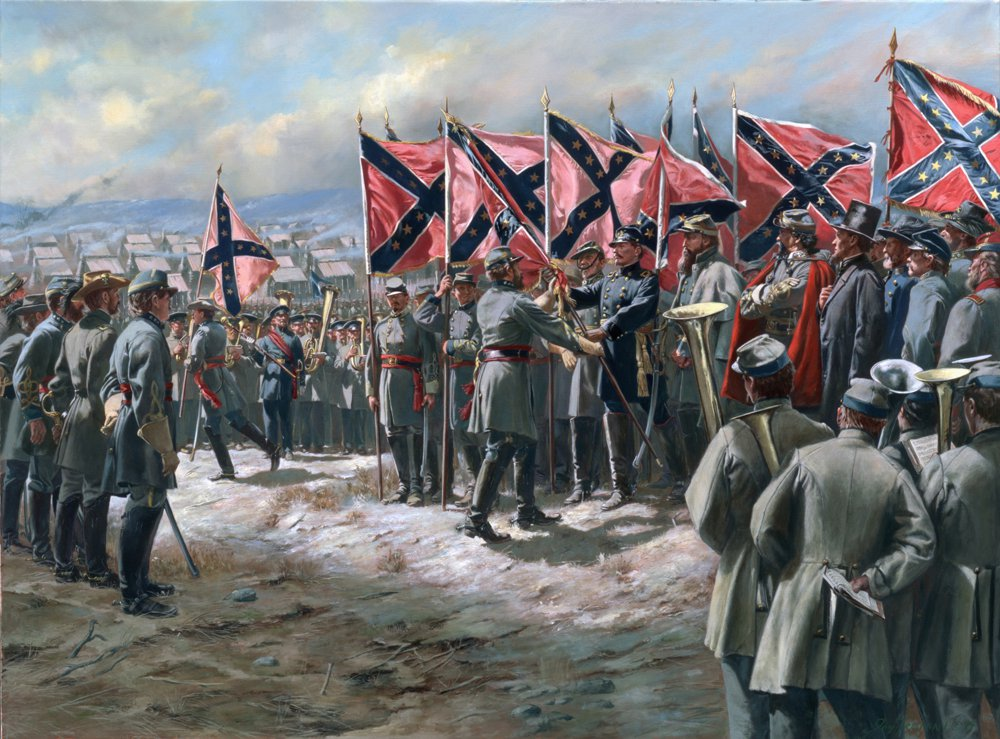
\includegraphics[width = 0.8\textwidth]{img/confederate}

\vspace{15pt}

Confederate Army in the US

\end{frame}
% ----------------------------------------------------

% ----------------------------------------------------
% \begin{frame}
% \frametitle{The universe of civil wars}
% \centering
%
% 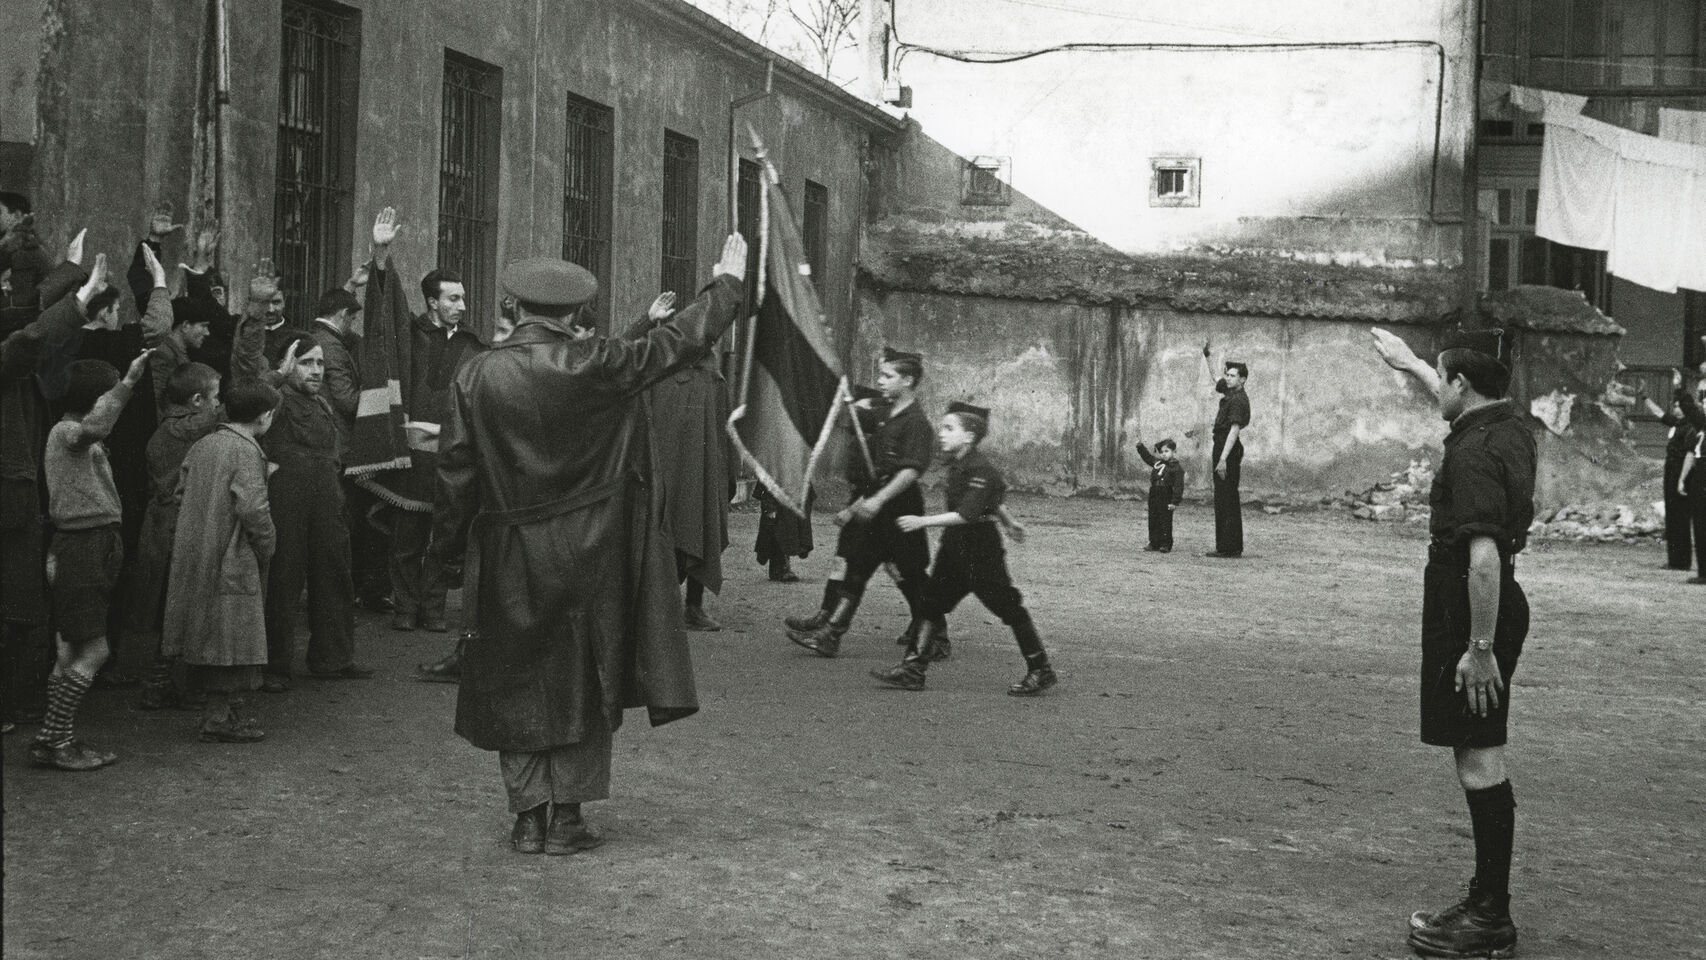
\includegraphics[width = 0.9\textwidth]{img/gv_oviedo}
%
% \vspace{15pt}
%
% Oviedo, 1937 (Spanish Civil War)
%
% \end{frame}
% % ----------------------------------------------------

% ----------------------------------------------------
\begin{frame}
\frametitle{The universe of civil wars}
\centering

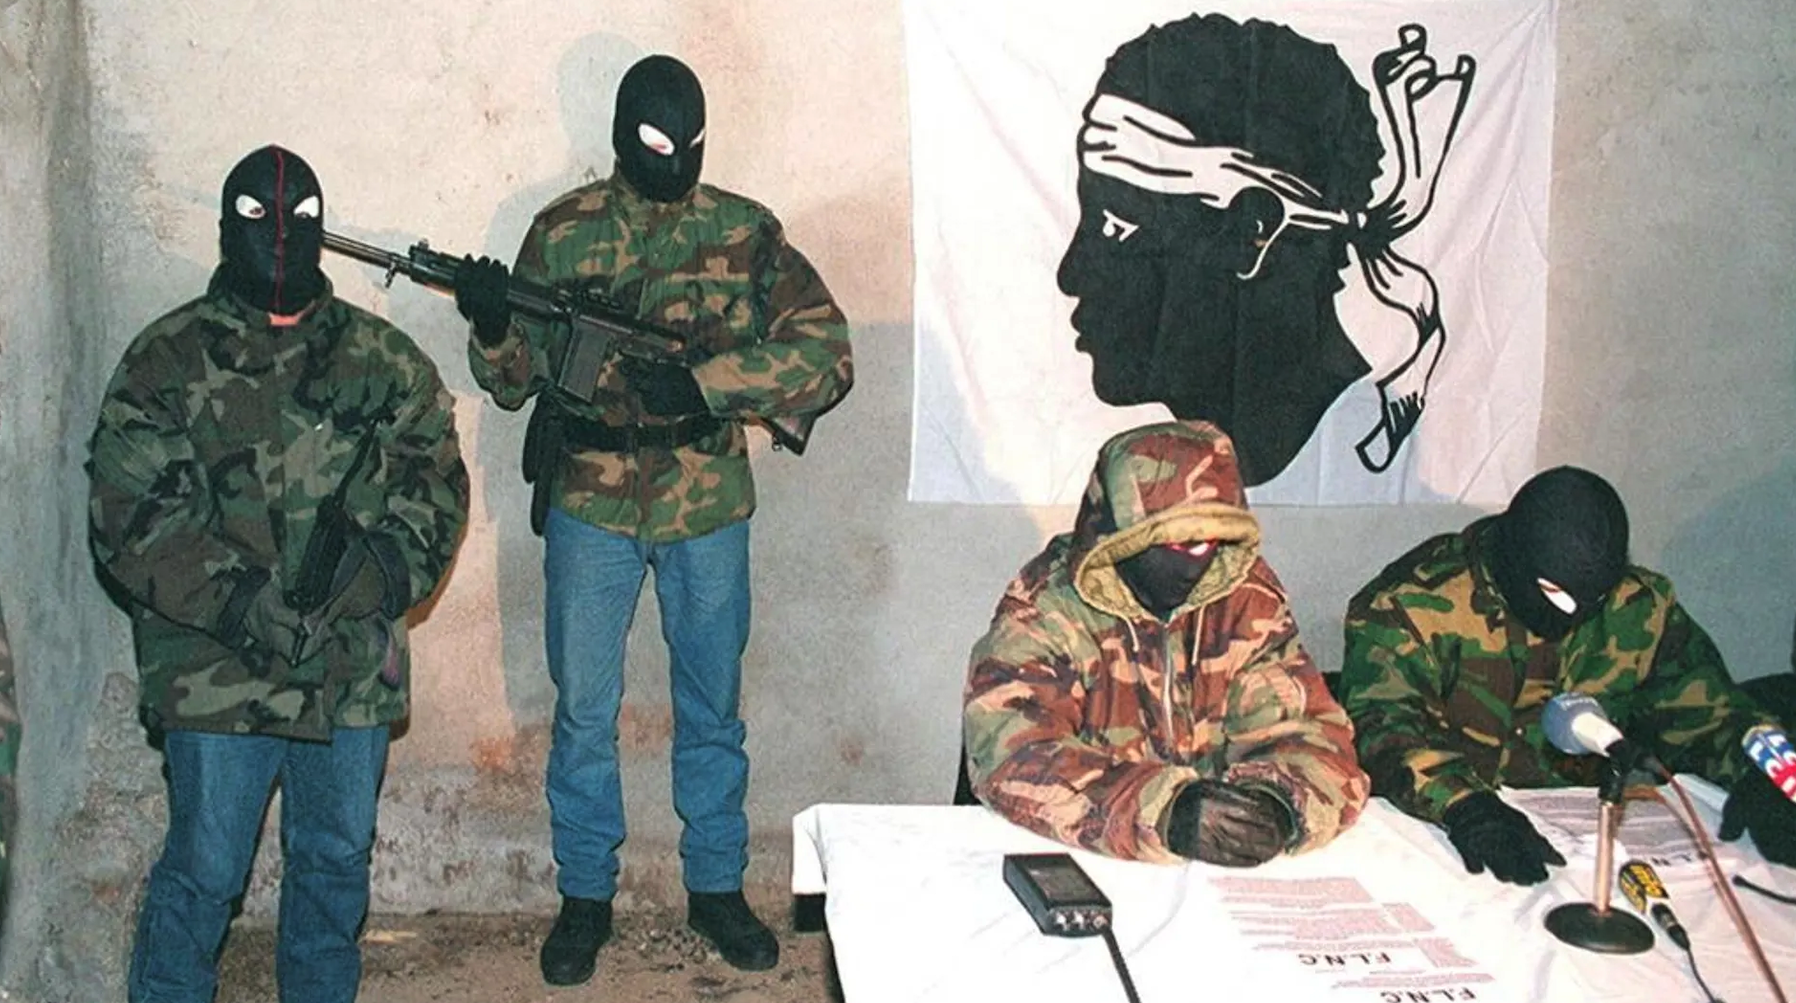
\includegraphics[width = 0.8\textwidth]{img/flnc}

FLNC in Corsica, France

\end{frame}
% ----------------------------------------------------

% ----------------------------------------------------
\begin{frame}
\frametitle{The universe of civil wars}
\centering

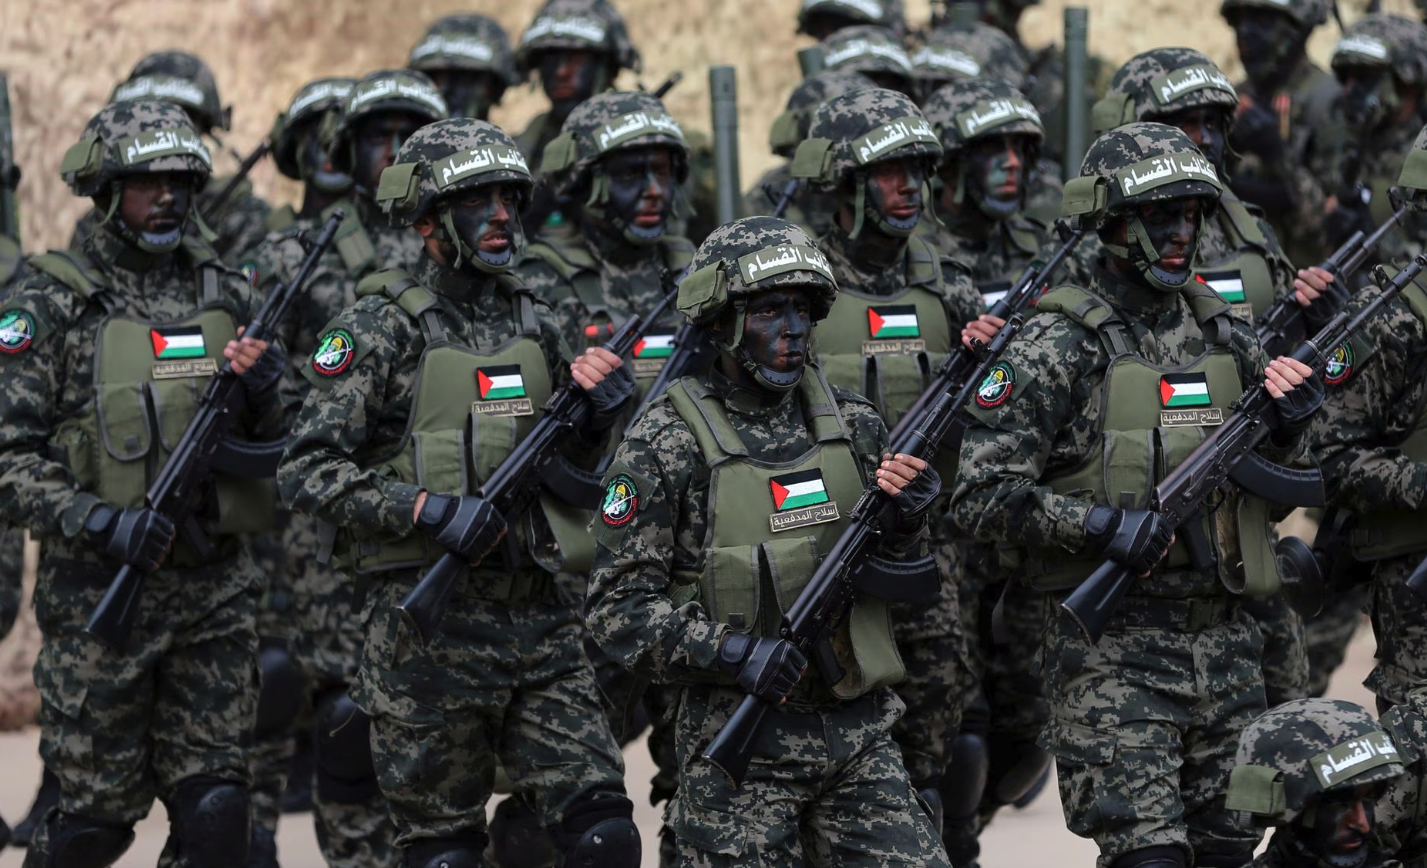
\includegraphics[width = 0.8\textwidth]{img/hamas}

Hamas in Gaza

\end{frame}
% ----------------------------------------------------

% ----------------------------------------------------
\begin{frame}
\frametitle{The universe of civil wars}
\centering

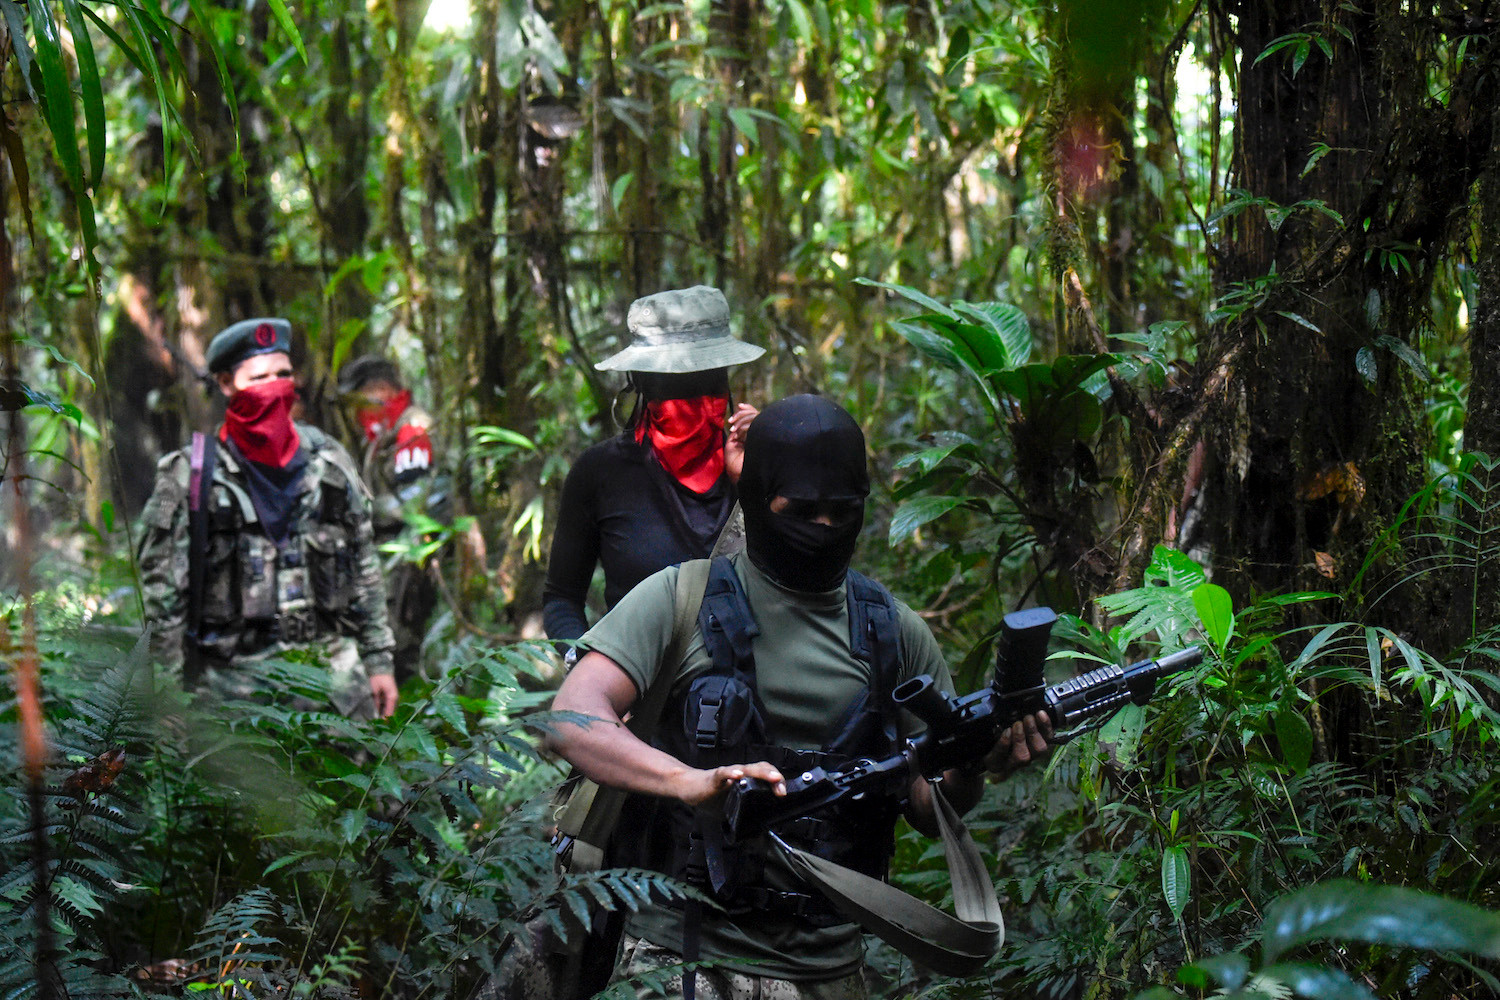
\includegraphics[width = 0.9\textwidth]{img/colombia}

\vspace{15pt}

ELN in Colombia

\end{frame}
% ----------------------------------------------------

% ----------------------------------------------------
\begin{frame}
\frametitle{The universe of civil wars}
\centering

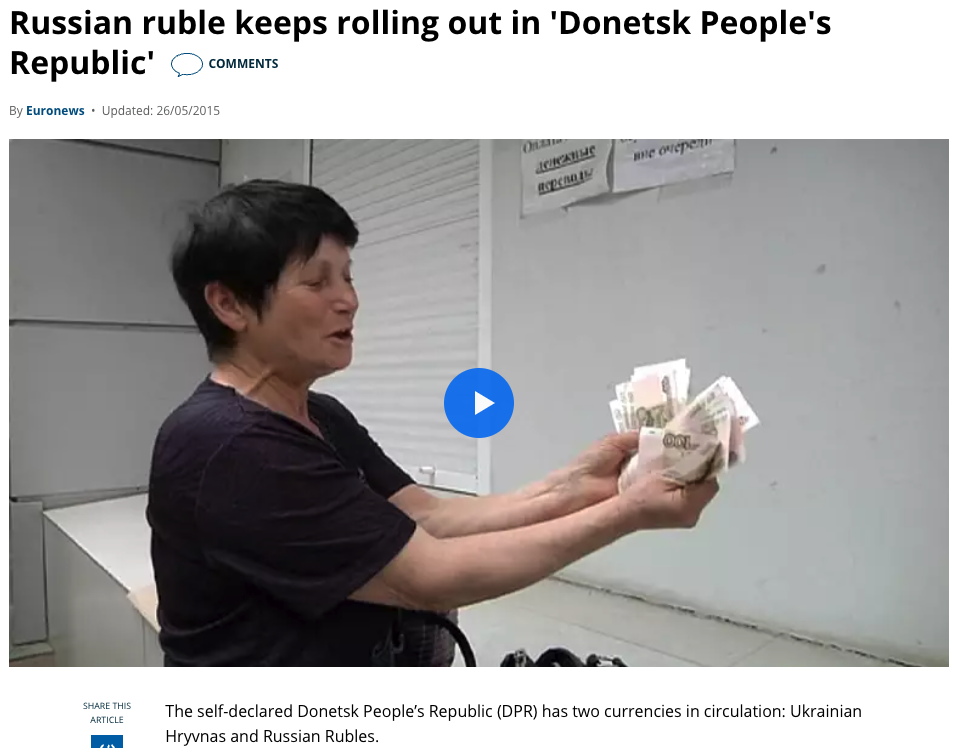
\includegraphics[width = 0.75\textwidth]{img/donbas}

\vspace{15pt}

Donetsk People's Republic

\end{frame}
% ----------------------------------------------------

% ----------------------------------------------------
\begin{frame}
\frametitle{The universe of civil wars}
\centering

\begin{itemize}
  \item We've seen this: civil wars look very different from each other
  \item Why?
  \item<2-> Much of this variation is due to differences in rebel groups
  \begin{itemize}
    \item All states usually share some characteristics
  \end{itemize}
  \item<3-> Think of them as \BGyellow{organizations}
  \item<4-> A few questions:
  \begin{itemize}
    \item<5->[1.] How do rebel groups vary? Do they change?
    \item<6->[2.] Why are they different?
    \item<7->[3.] What consequences do these differences have? (their behavior)
  \end{itemize}
\end{itemize}

\end{frame}
% ----------------------------------------------------

% ----------------------------------------------------
\begin{frame}
\frametitle{The universe of \BGyellow{rebel organizations}}
\centering

\begin{itemize}
  \item Think about differences across rebel groups
  \item How are they different?
  \begin{itemize}
    \item<2-> `technology of insurgency'
    \item<3-> recruitment
    \item<4-> patterns of violence
    \item<5-> ideology
    \item<6-> constituency
    \item<7-> internal organization
    \item<8-> alliances
    \item<8-> ...
  \end{itemize}
  \item<9-> If you think about these, some refer to \textbf{actions} and some to \textbf{characteristics}
\end{itemize}

\end{frame}
% ----------------------------------------------------


% ----------------------------------------------------
\begin{frame}
\frametitle{The universe of \BGyellow{rebel organizations}}
\centering

\begin{itemize}
  \item One more important aspect: \textbf{wartime governance} of civilians
  \begin{itemize}
    \item<2-> Whether and how rebel groups interact with local civilians
    \item<3-> Not directly related to warfare
    \item<4-> Not talking about violence here (only, at least)
  \end{itemize}
\end{itemize}

\end{frame}
% ----------------------------------------------------

% ----------------------------------------------------
\begin{frame}
\frametitle{Rebel governance}
\centering

\begin{itemize}
  \item<1-> Wars are \textbf{not} continuous and non-stop violence and anarchy
  \item<2-> \textbf{Rebels} make a \textbf{decision} on how to rule local civilians, and \textbf{civilians} also have some \textbf{influence} on how they are ruled
  \item<3-> This \BGyellow{`wartime social order'} can be purely coercive and violent, but most groups engage in some form of governance:
  \begin{itemize}
    \item taxation, popular assemblies, courts, schools, etc
  \end{itemize}
\end{itemize}

\end{frame}
% ----------------------------------------------------

% ----------------------------------------------------
\begin{frame}
\frametitle{Sri Lankan civil war (1983--2009)}
\centering

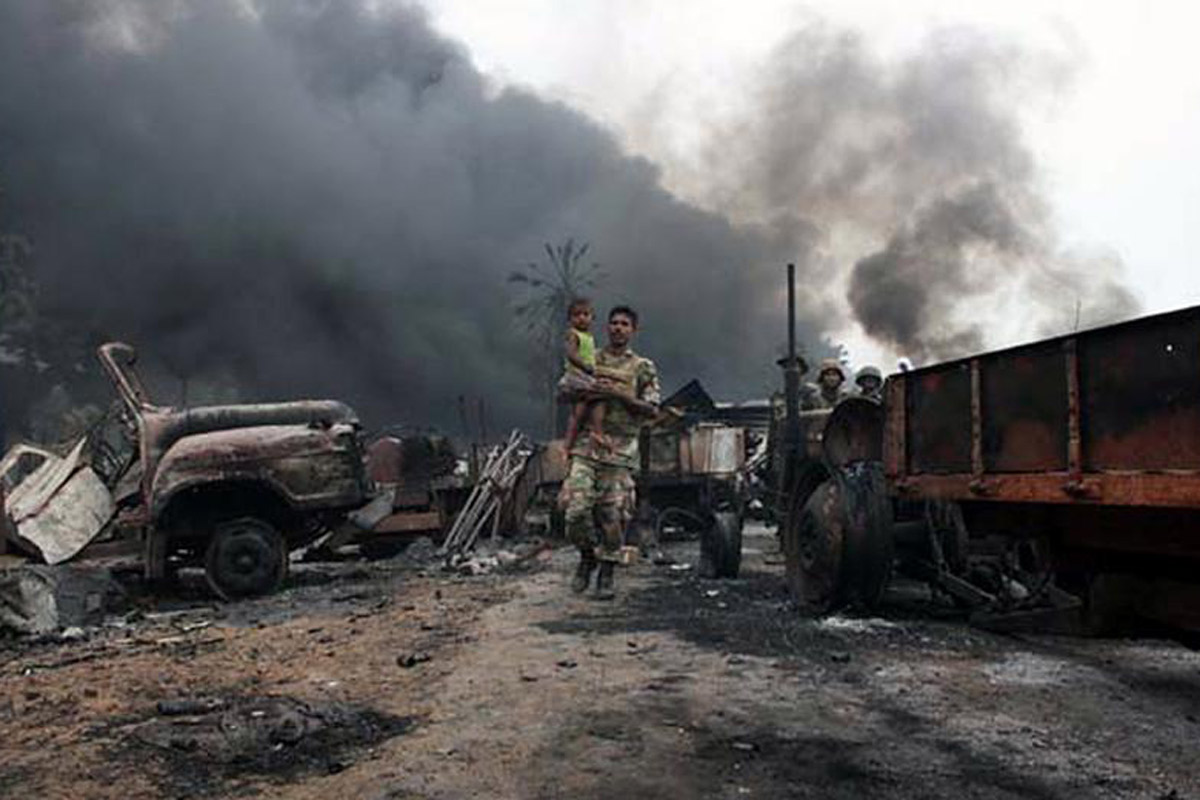
\includegraphics[width = 0.8\textwidth]{img/sri_lanka_war}

\end{frame}
% ----------------------------------------------------

% ----------------------------------------------------
\begin{frame}
\frametitle{LTTE (Liberation Tigers of Tamil Eelam)}
\centering

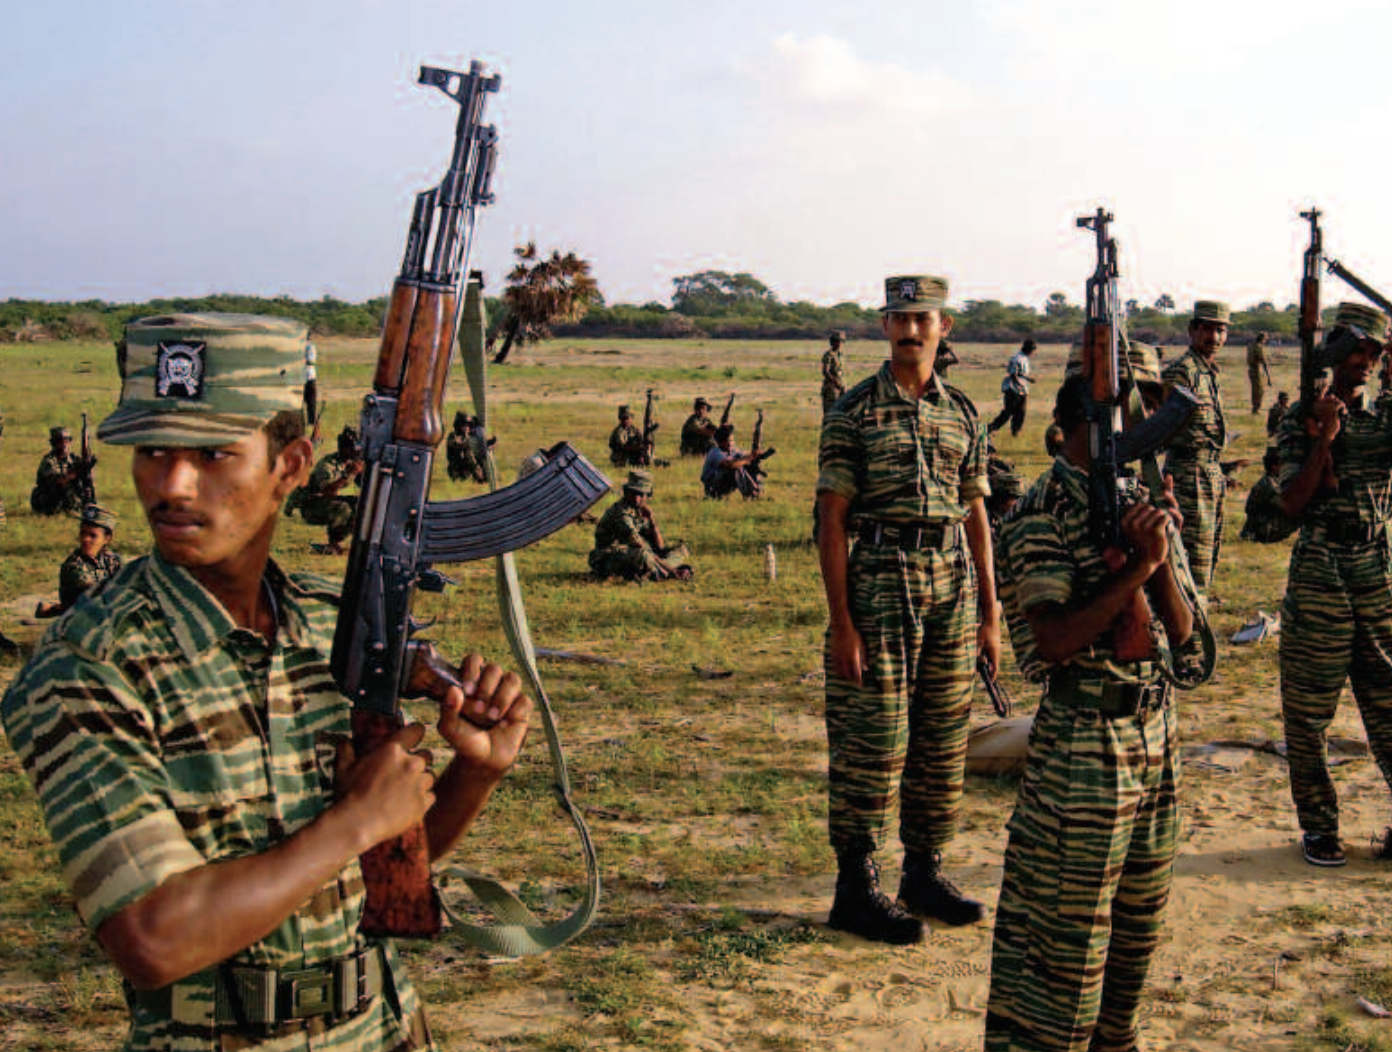
\includegraphics[width = 0.8\textwidth]{img/ltte}

\end{frame}
% ----------------------------------------------------

% ----------------------------------------------------
\begin{frame}
\frametitle{LTTE \& civilian governance}
\centering

\begin{minipage}{0.4\textwidth}\centering
  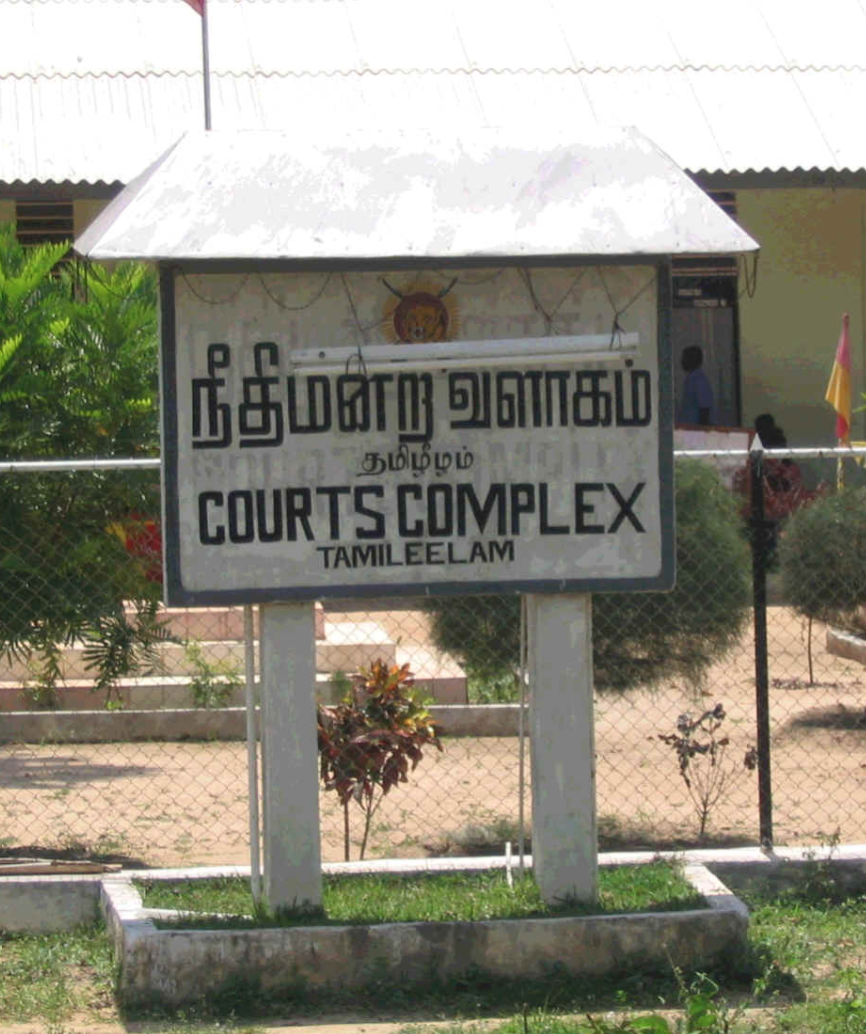
\includegraphics[width = 0.9\textwidth]{img/tamileelam_courts}
  \vfill
\end{minipage}\hfill
\begin{minipage}{0.59\textwidth}\centering
  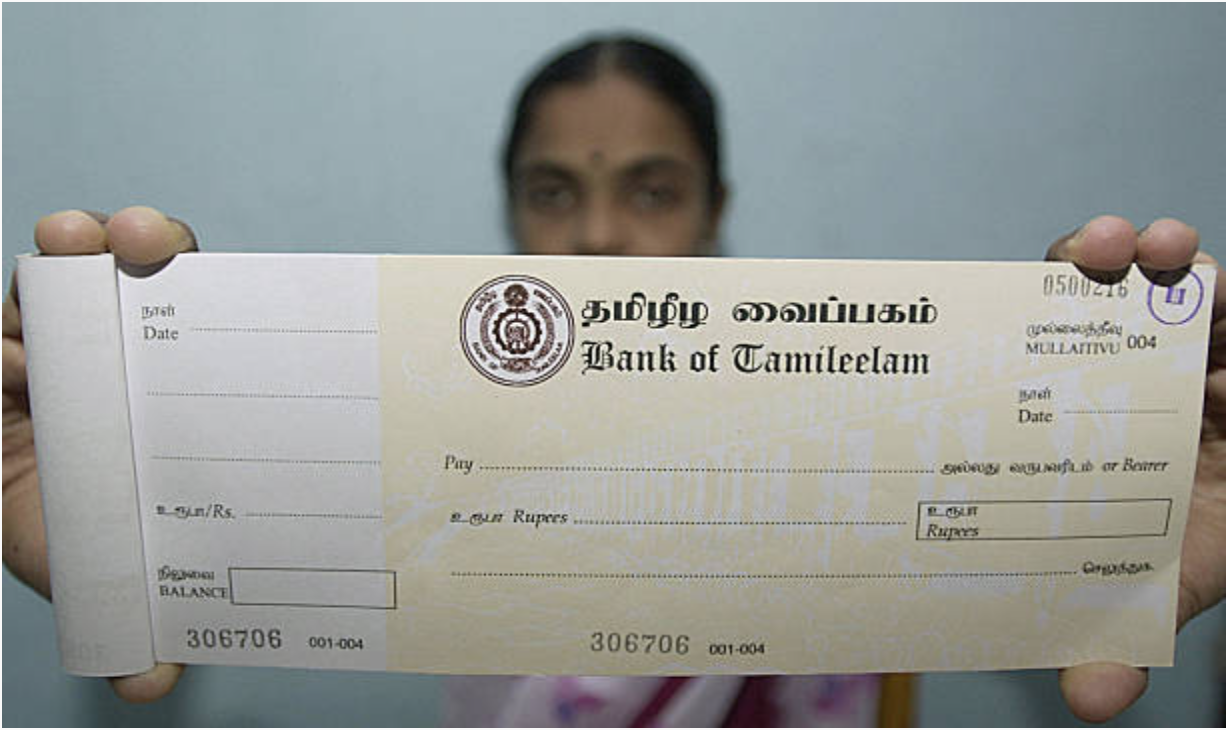
\includegraphics[width = \textwidth]{img/tamileelam_bank}\\
  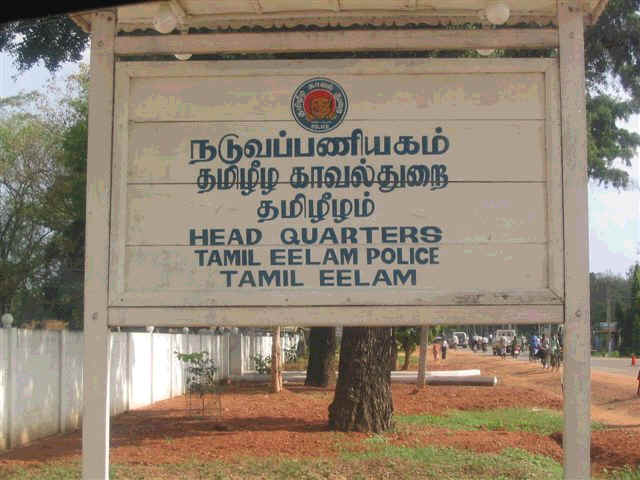
\includegraphics[width = .8\textwidth]{img/tamileelam_police}
\end{minipage}

\end{frame}
% ----------------------------------------------------

% ----------------------------------------------------
\begin{frame}
\frametitle{Understand governance}
\centering

\begin{itemize}
  \item<1-> A civil war is a conflict over control of territory and \textit{people}
  \begin{itemize}
    \item A crucial aspect: \textbf{civilian collaboration}
  \end{itemize}
  \item<2-> Civilians offer opportunities to the rebels (recruits, material support, information, etc) but \textbf{can also defect} to the enemy
  \item<3-> \BGyellow{Rebel governance} is developed to win over the support of the local population and disincentivize collaboration with the enemy
  \begin{itemize}
    \item<4-> Very dependent on territorial control (you can't obviously build banks or bureaucracies if you are a guerrilla group without firm territorial control)
  \end{itemize}
\end{itemize}

\end{frame}
% ----------------------------------------------------

% ----------------------------------------------------
\begin{frame}
\frametitle{Rebel governance}
\centering

\begin{itemize}
  \item But \BGyellow{why} do groups differ on how their relate to civilians?
\end{itemize}

\end{frame}
% ----------------------------------------------------

% ----------------------------------------------------
\begin{frame}
\frametitle{Greed perspective: Resources and control}
\centering

\begin{minipage}{0.49\textwidth}\centering
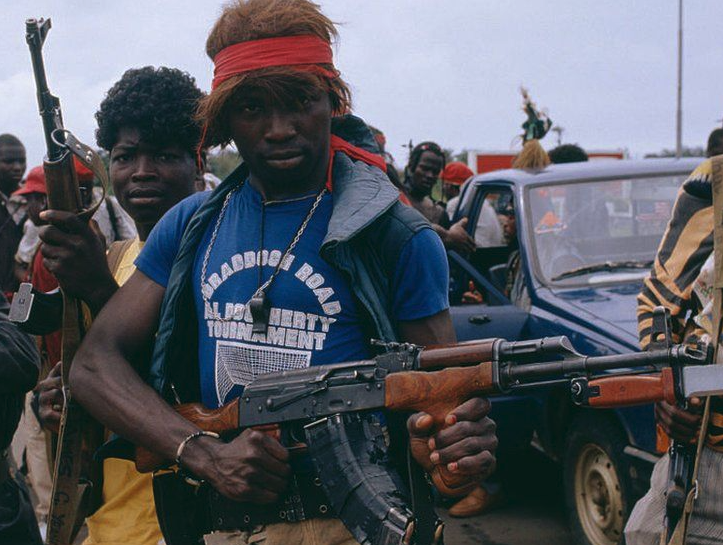
\includegraphics[width = \textwidth]{img/liberia}\\Charles Taylor's NPFL in Liberia
\end{minipage}\hfill
\begin{minipage}{0.49\textwidth}\centering
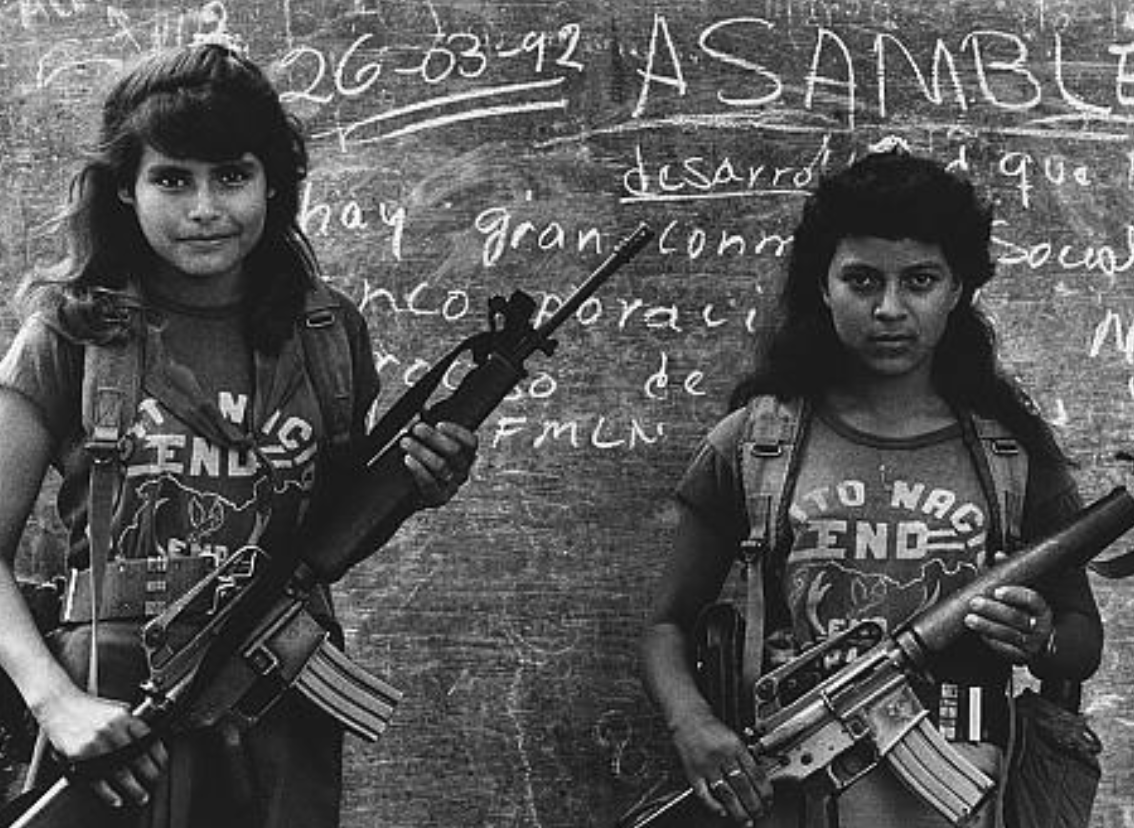
\includegraphics[width = \textwidth]{img/fmln}\\FNML in El Salvador
% {\small Jeremy Weinstein (2007)}
\end{minipage}

\end{frame}
% ----------------------------------------------------

% ----------------------------------------------------
\begin{frame}
\frametitle{Greed perspective: Resources and control}
\centering

\begin{minipage}{0.6\textwidth}\centering
  \begin{itemize}[<+->]
    \item Why do some groups use violence while other restrain themselves?
    \item It depends on the initial conditions faced by rebel leaders:
    \item[1.] Do you have natural resources or foreign funding? No need for civilian cooperation, rule by the sword
    \item[2.] Do you need `social endowments'? You need to win `hearts and minds'
  \end{itemize}
\end{minipage}\hfill
\begin{minipage}{0.39\textwidth}\centering
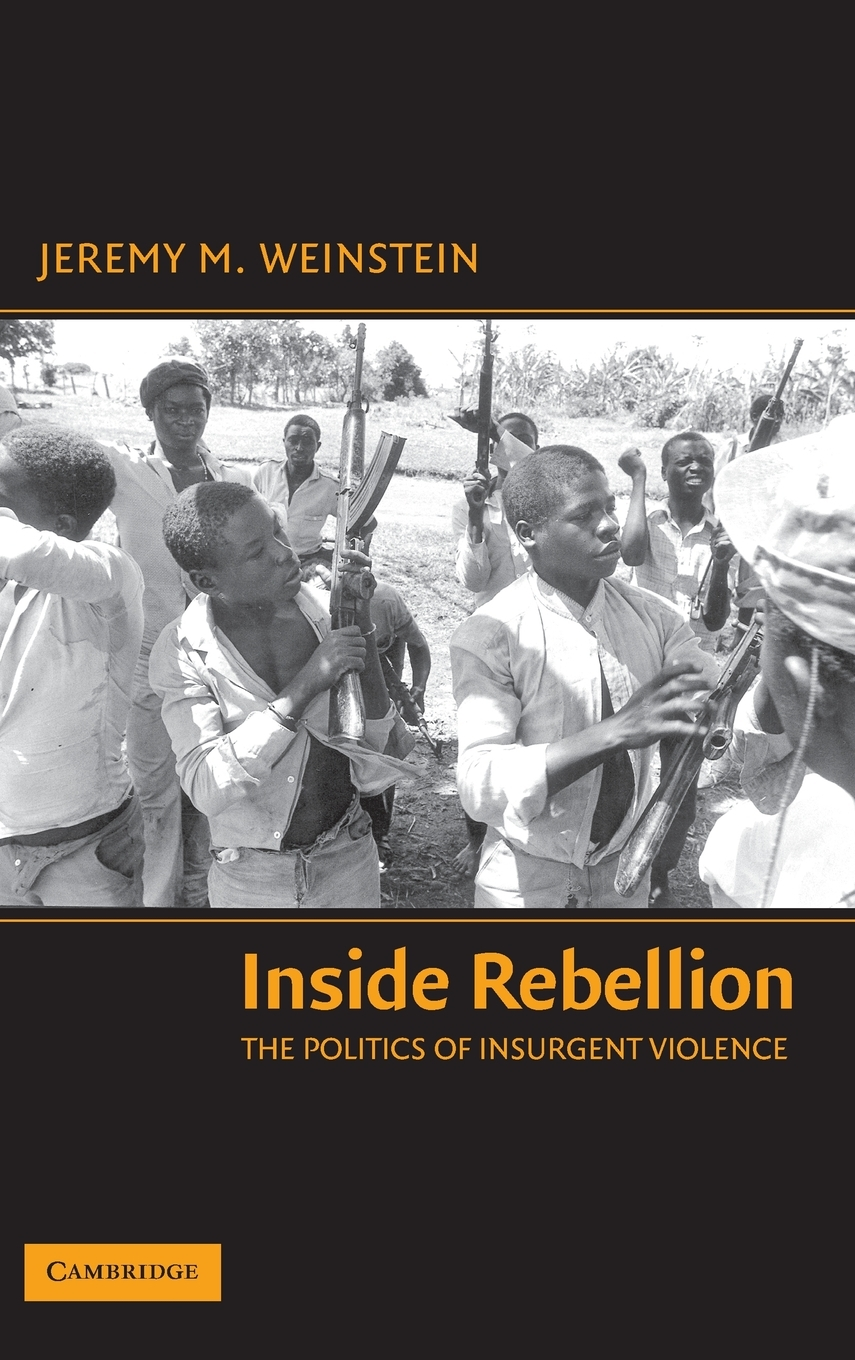
\includegraphics[width = 0.8\textwidth]{img/weinstein2007}\\
{\small Jeremy Weinstein (2007)}
\end{minipage}

\end{frame}
% ----------------------------------------------------

% ----------------------------------------------------
\begin{frame}
\frametitle{What about ISIS?}
\centering

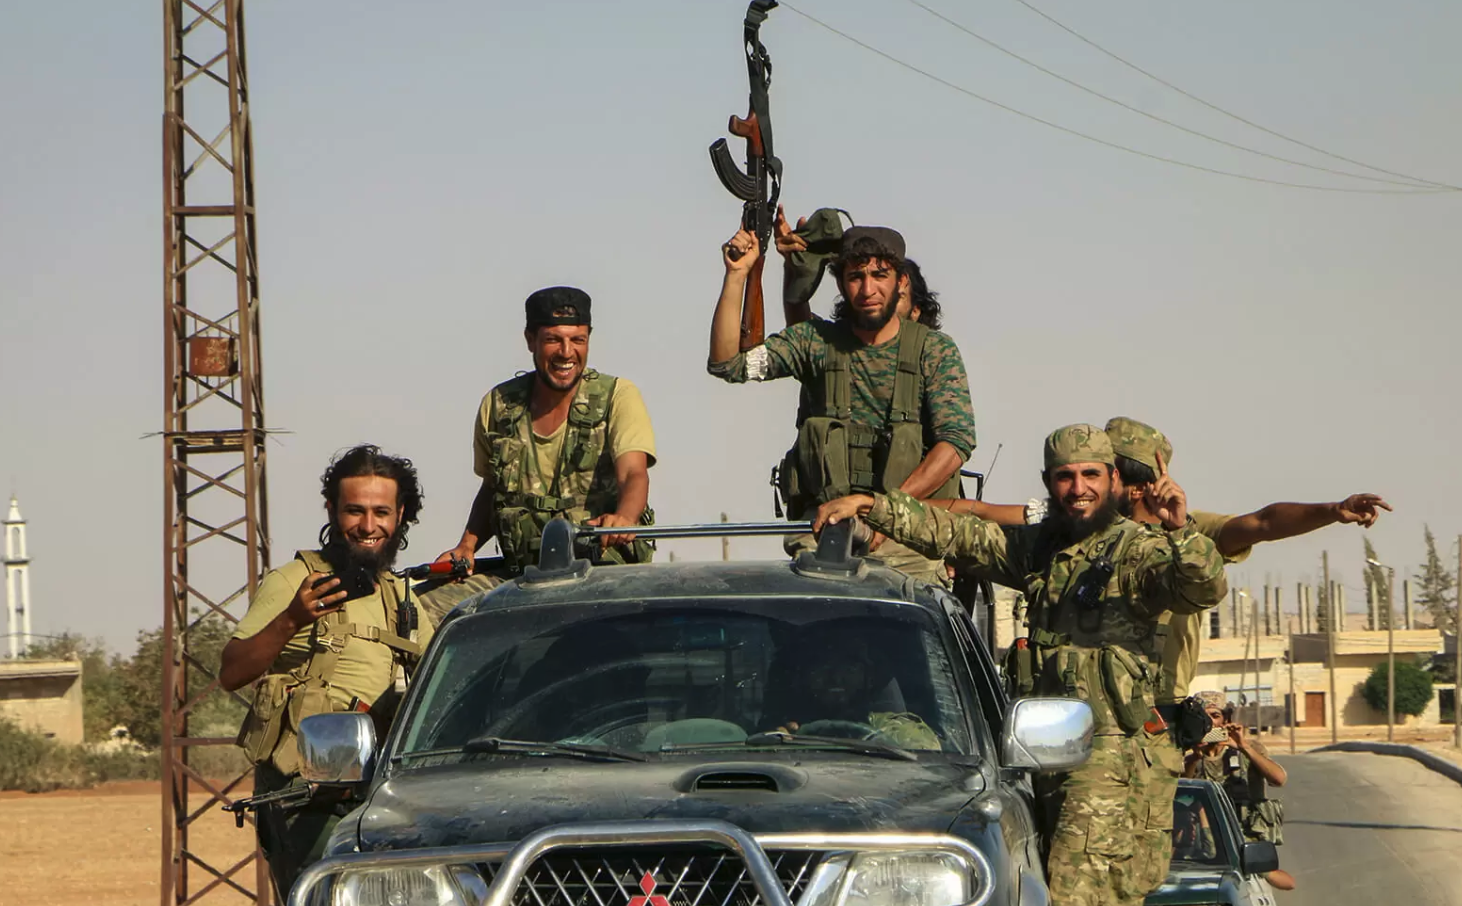
\includegraphics[width = \textwidth]{img/isis}

\end{frame}
% ----------------------------------------------------

% ----------------------------------------------------
\begin{frame}
\frametitle{What about ISIS?}
\centering

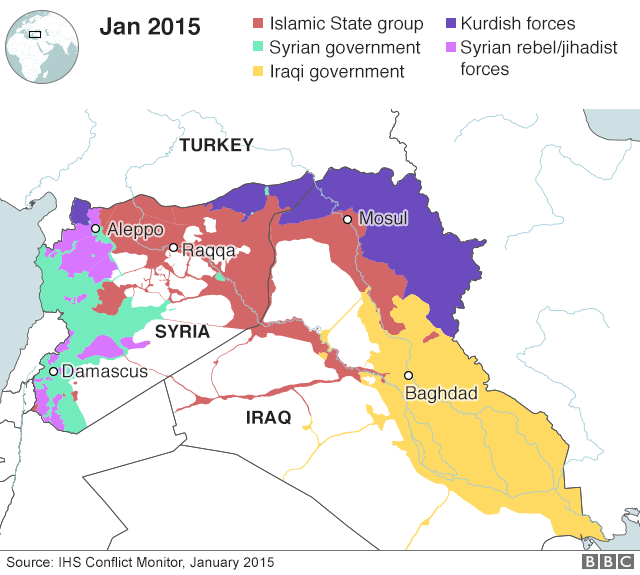
\includegraphics[width = 0.7\textwidth]{img/isis_terrctrl}

\end{frame}
% ----------------------------------------------------

% ----------------------------------------------------
\begin{frame}
\frametitle{What about ISIS?}
\centering

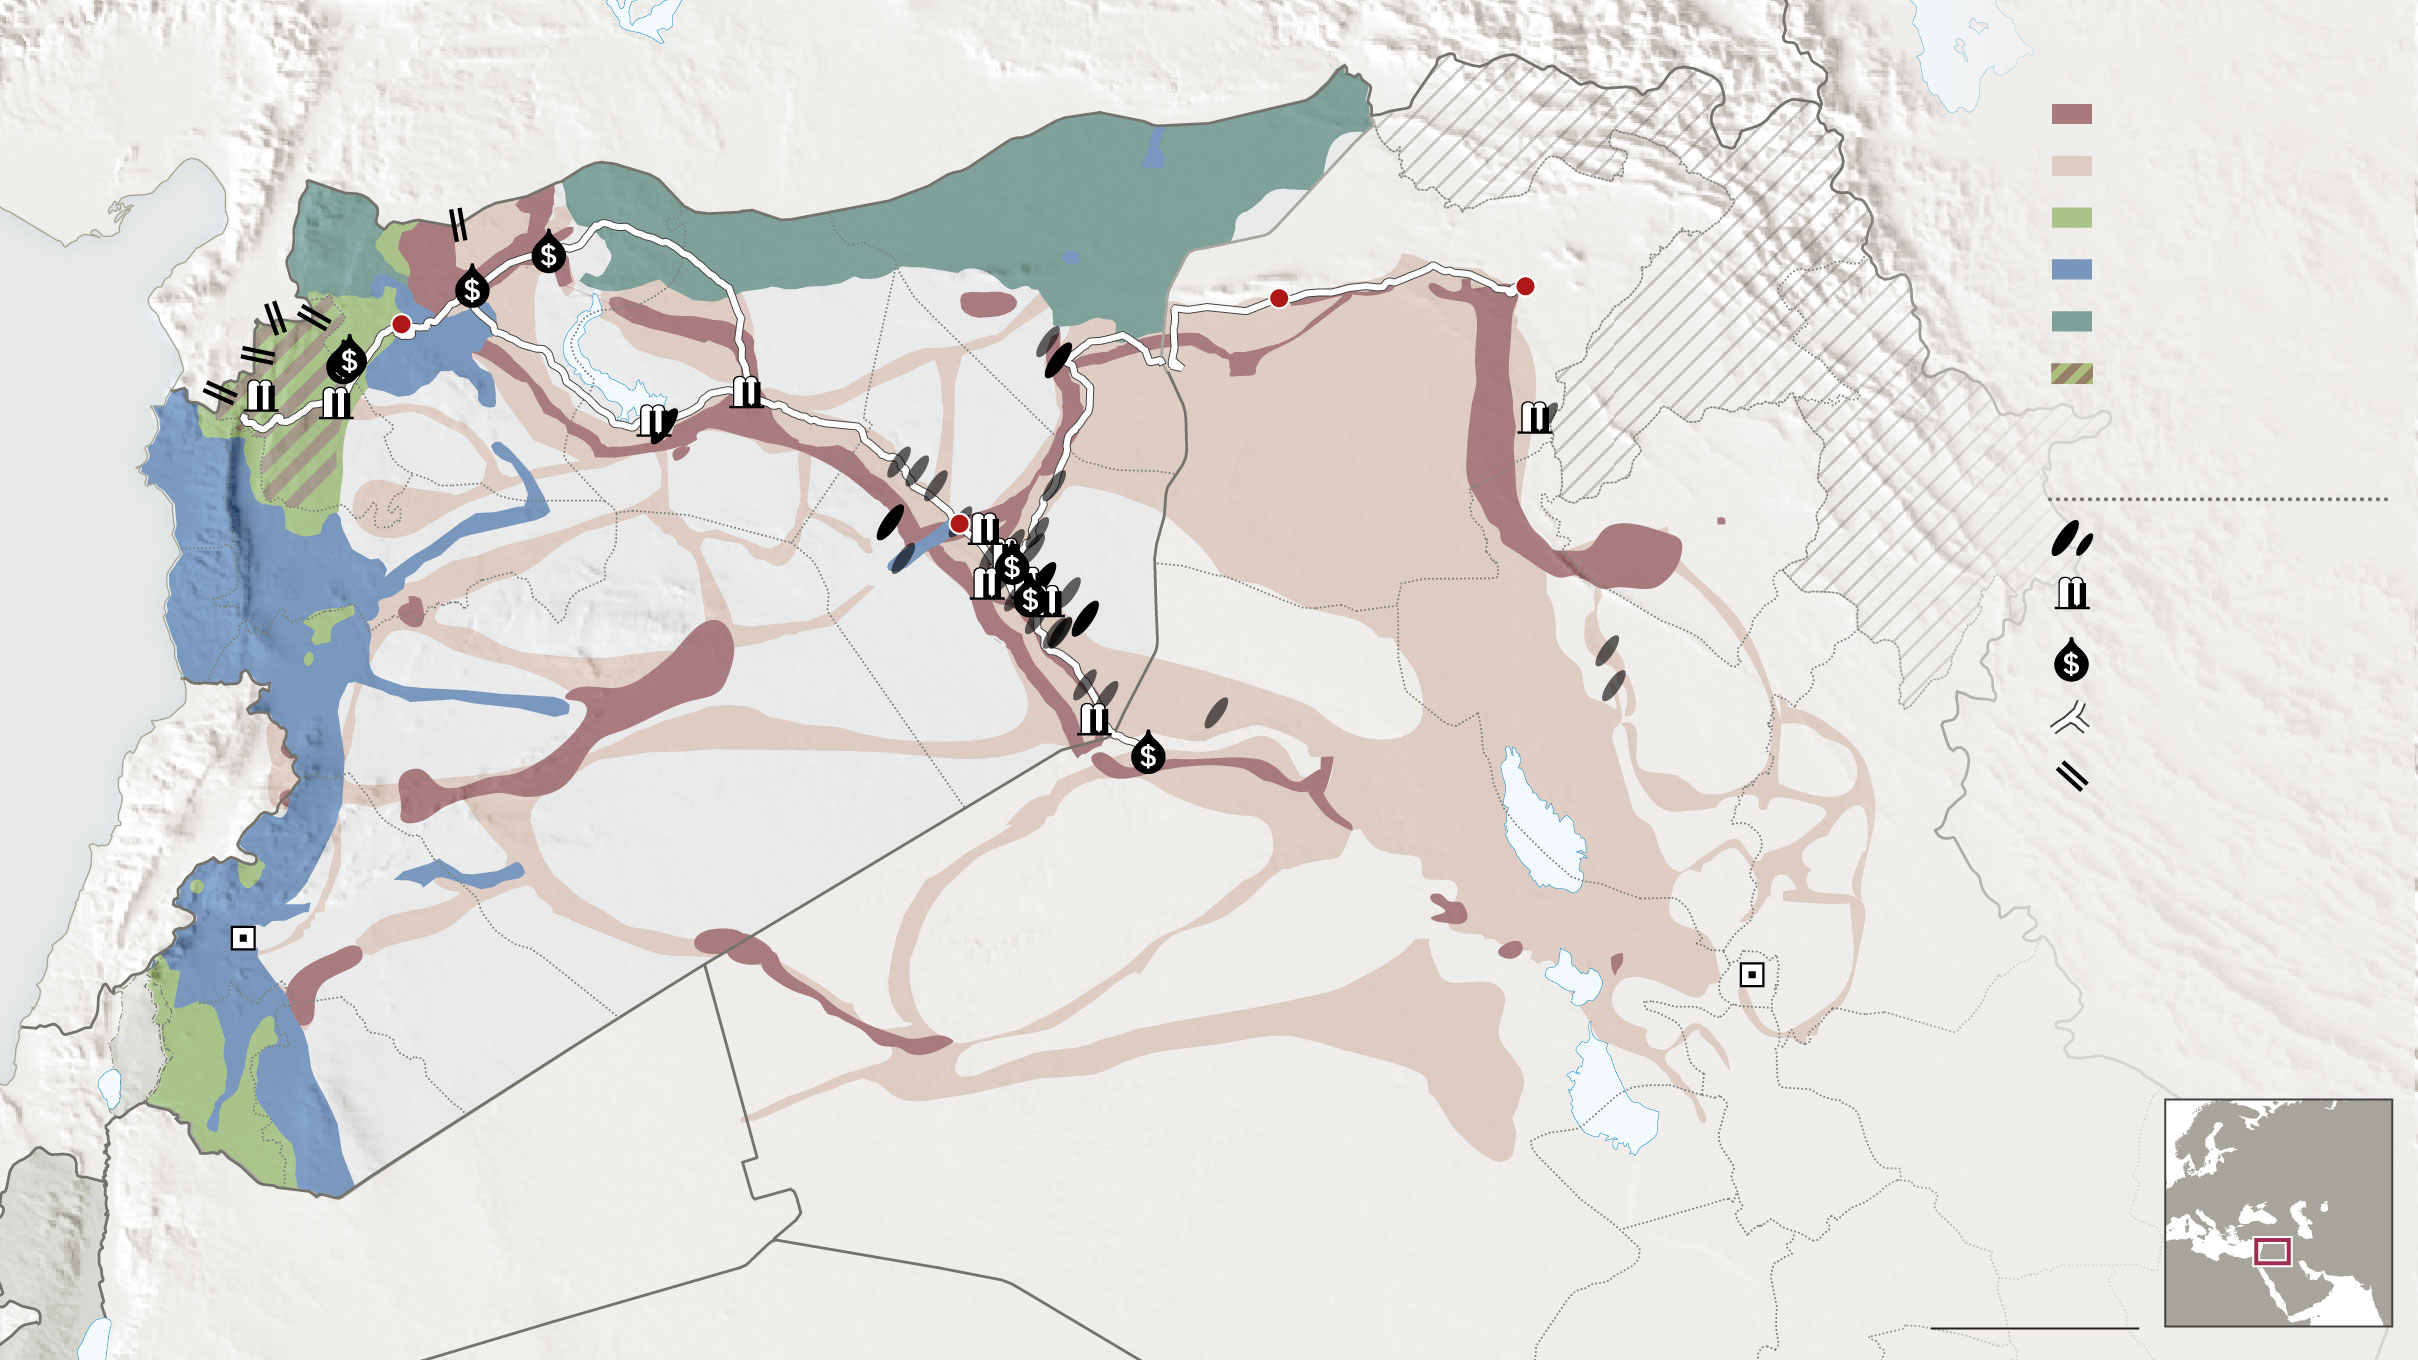
\includegraphics[width = \textwidth]{img/isis_syria_oil}

\begin{itemize}
  \item What would you expect from ISIS?
\end{itemize}


\end{frame}
% ----------------------------------------------------

% ----------------------------------------------------
\begin{frame}
\frametitle{Resources and control: ISIS?}
\centering

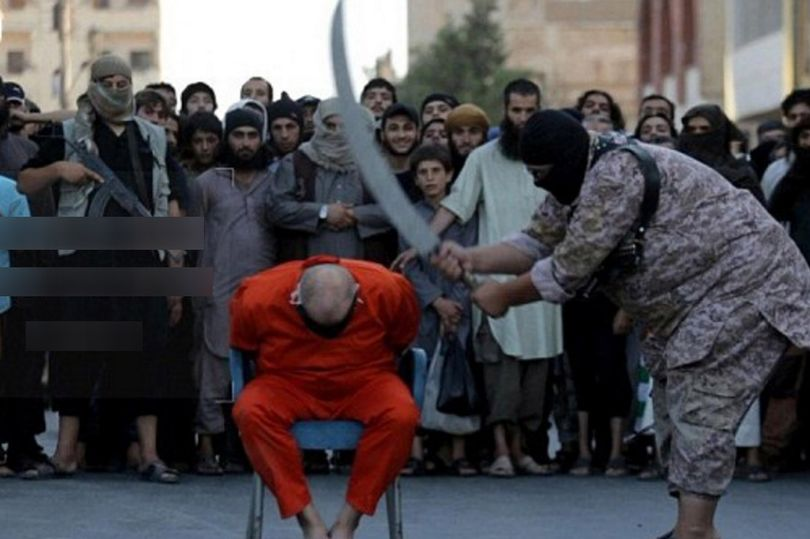
\includegraphics[width = 0.7\textwidth]{img/isis-raqqa}

\vspace{15pt}

ISIS public execution in Raqqa (Syrian Civil War)

\end{frame}
% ----------------------------------------------------

% ----------------------------------------------------
\begin{frame}
\frametitle{Resources and control: ISIS?}
\centering

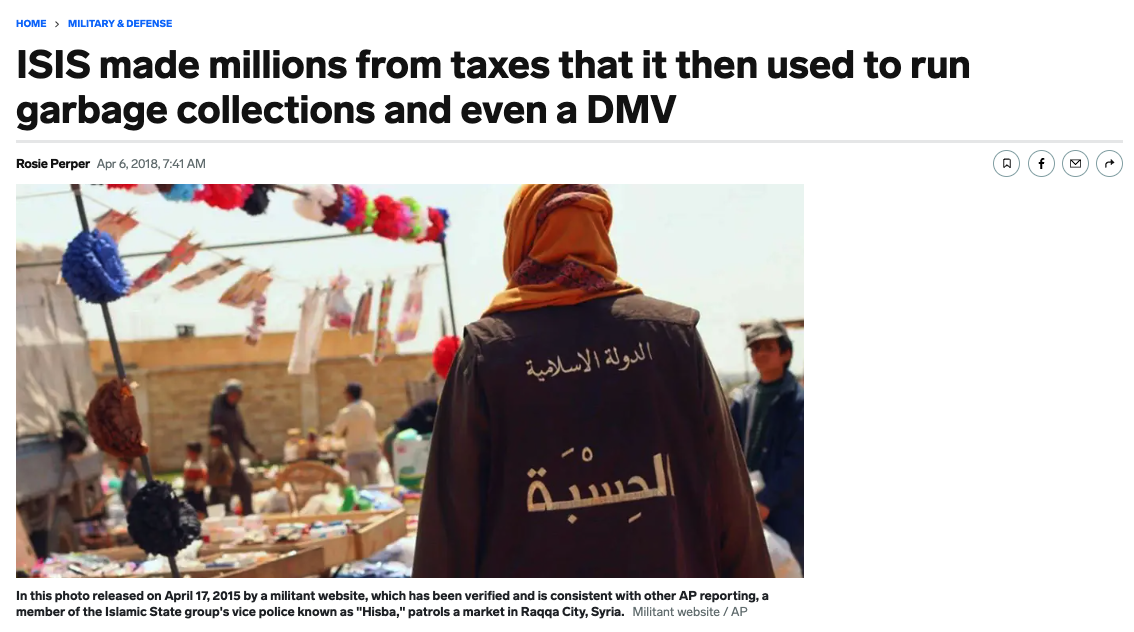
\includegraphics[width = \textwidth]{img/isis_taxing}

\end{frame}
% ----------------------------------------------------

% ----------------------------------------------------
\begin{frame}
\frametitle{Resources and control: ISIS?}
\centering

\begin{itemize}
  \item So why would an oil-rich group as ISIS engage in costly governance?
  \item<2-> The role of \BGyellow{ideology}, not only material incentives
  \begin{itemize}
    \item Which also explains many other aspects of rebel governance
  \end{itemize}
  \item<3-> \BGyellow{War pressures}
  \begin{itemize}
    \item Similar to Tilly's state formation idea
  \end{itemize}
  \end{itemize}

\end{frame}
% ----------------------------------------------------


% ----------------------------------------------------
\begin{frame}
\frametitle{Understanding rebel governance}
\centering

\begin{itemize}[<+->]
  \item Rebel organizations need to enforce collaboration
  \item But violence alone is \textbf{never enough}, nor are just private, financial incentives
  \begin{itemize}
    \item example of private incentives?
  \end{itemize}
  \item Given some degree of territorial control, some rebel governance usually exists
  \item But its \textbf{shape varies} a lot, which depends on several factors:
  \begin{itemize}
    \item Prewar cultural and political norms
    \item Problems that appear during the war
    \item Influence of local civilians
    \item Imitation of state symbols and practices
  \end{itemize}
  \item Some focus on economic production, health, education, some develop more participatory institutions, etc
\end{itemize}

\end{frame}
% ----------------------------------------------------

% ----------------------------------------------------
\begin{frame}
\frametitle{Understanding rebel governance}
\centering

\begin{minipage}{0.7\textwidth}\centering
  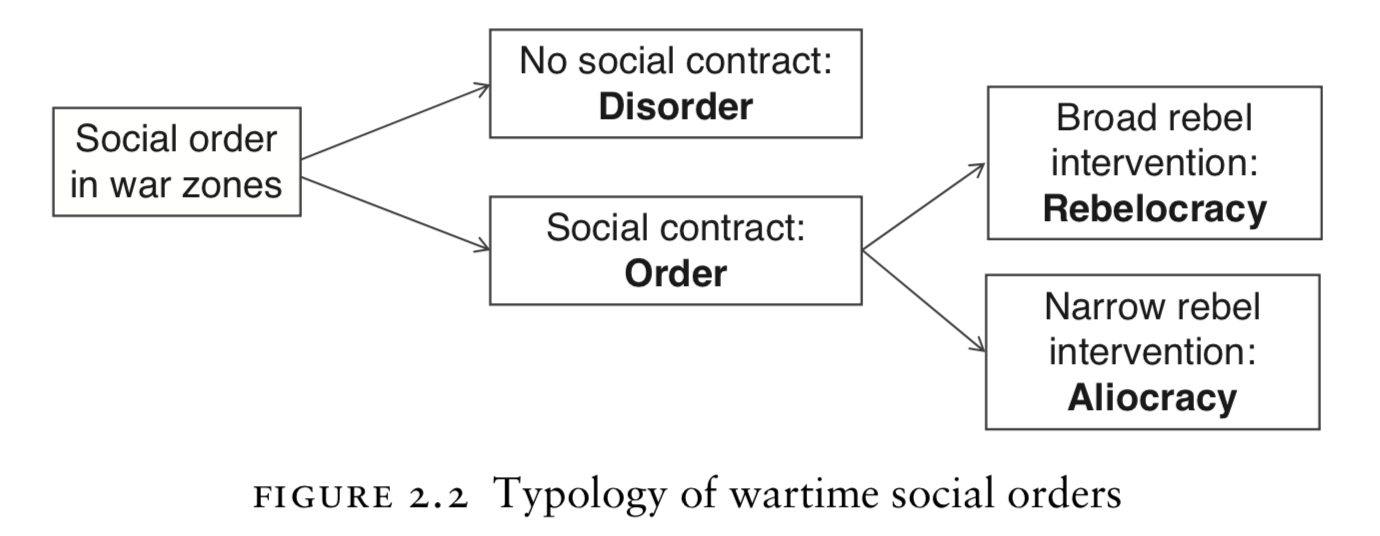
\includegraphics[width = \textwidth]{img/arjona_typology}\\\vspace{10pt}
  \begin{itemize}[<+->]
    \item[] {\footnotesize (\textit{Social contract} $\approx$ laws)}
    \item Rebel groups try to mazimize territorial control and what they get out of it
    \item Therefore, they should prefer order to disorder, and more intervention (rebelocracy) than less (aliocracy)
  \end{itemize}
\end{minipage}\hfill
\begin{minipage}{0.29\textwidth}\centering
  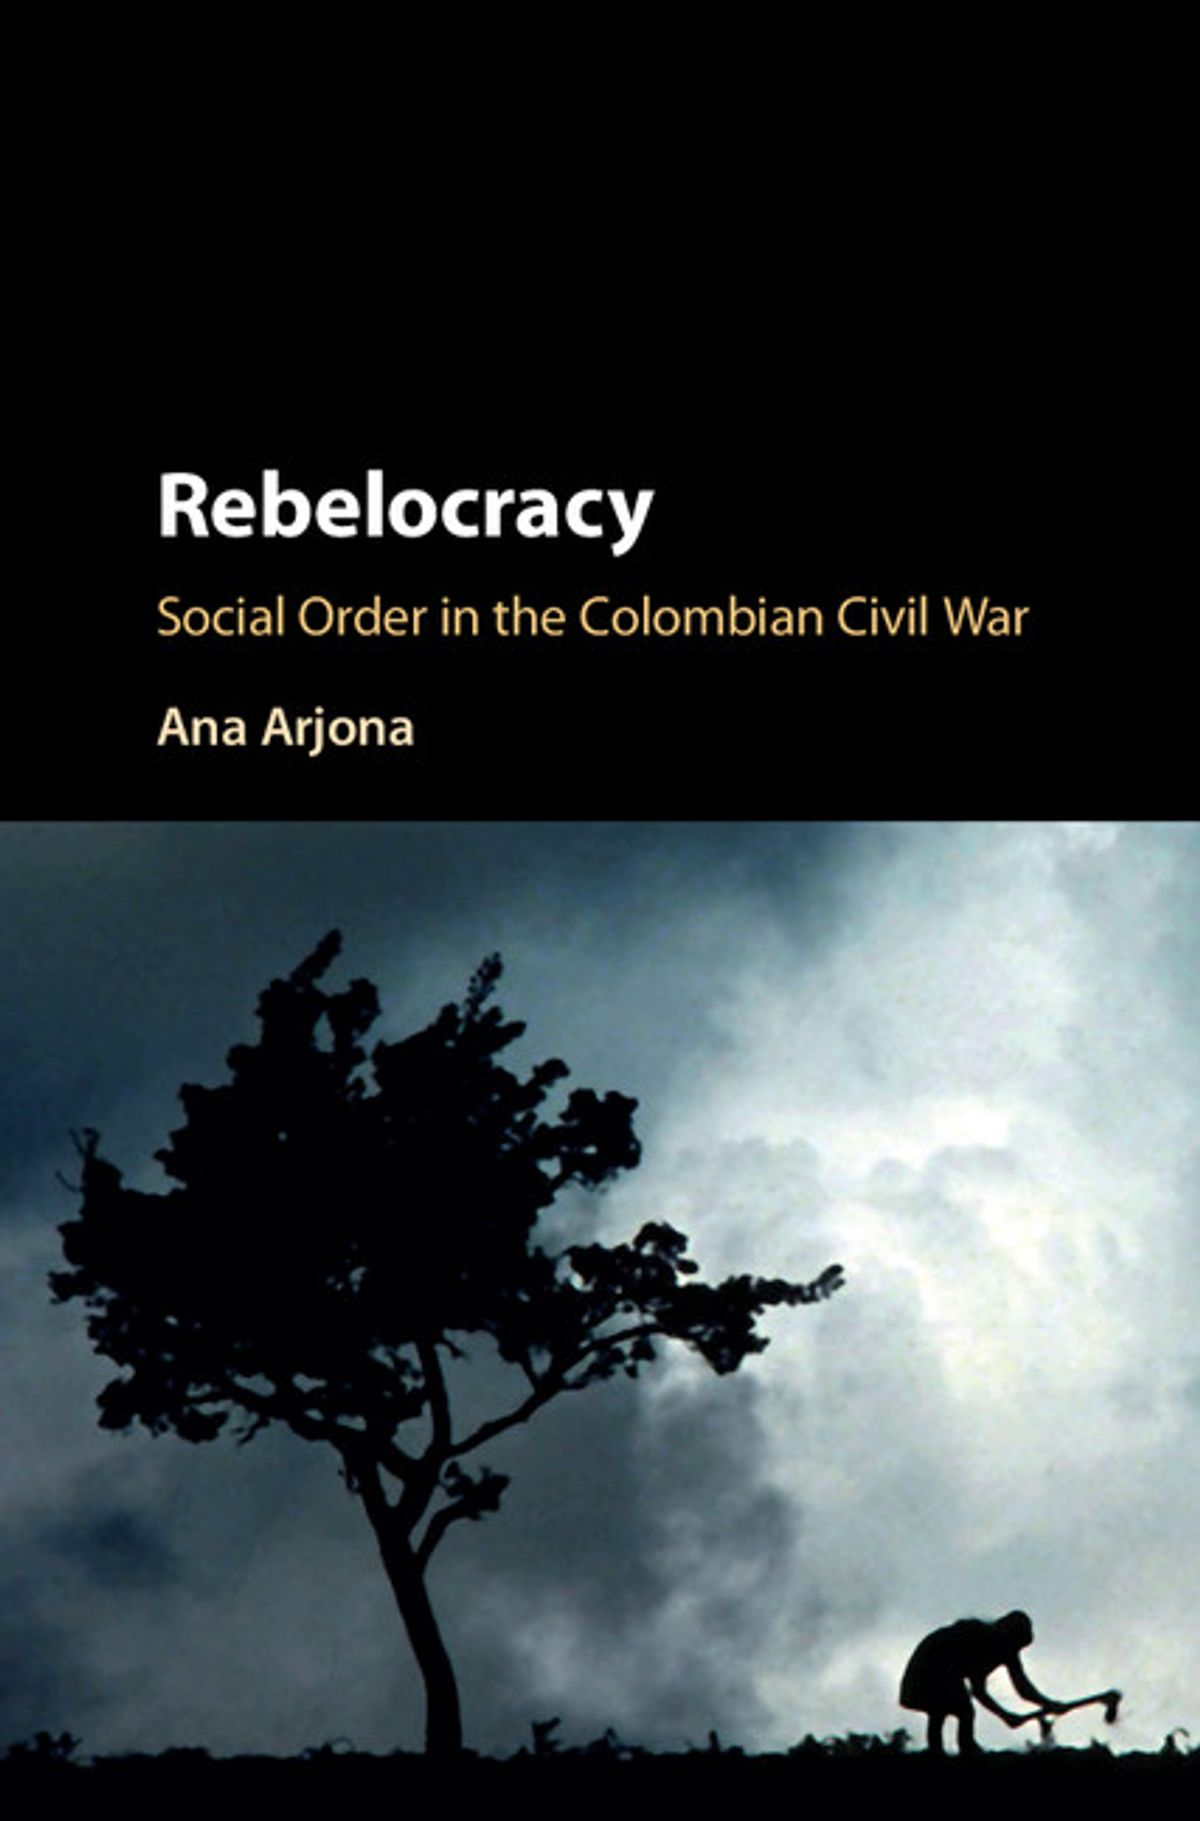
\includegraphics[width = 0.85\textwidth]{img/arjona_rebelocracy}\\
  {\small Ana Arjona (2017)}
\end{minipage}

\end{frame}
% ----------------------------------------------------

% ----------------------------------------------------
\begin{frame}
\frametitle{Understanding rebel governance}
\centering

% \begin{minipage}{0.7\textwidth}\centering
  \begin{itemize}
    \item When does \textbf{order and rebelocracy} emerge? (i.e. when do rebel engage in extensive governance?)
    \item Depends on the rebels' \BGyellow{time horizon and prewar local institutions}
  \end{itemize}
% \end{minipage}\hfill
% \begin{minipage}{0.29\textwidth}\centering
%   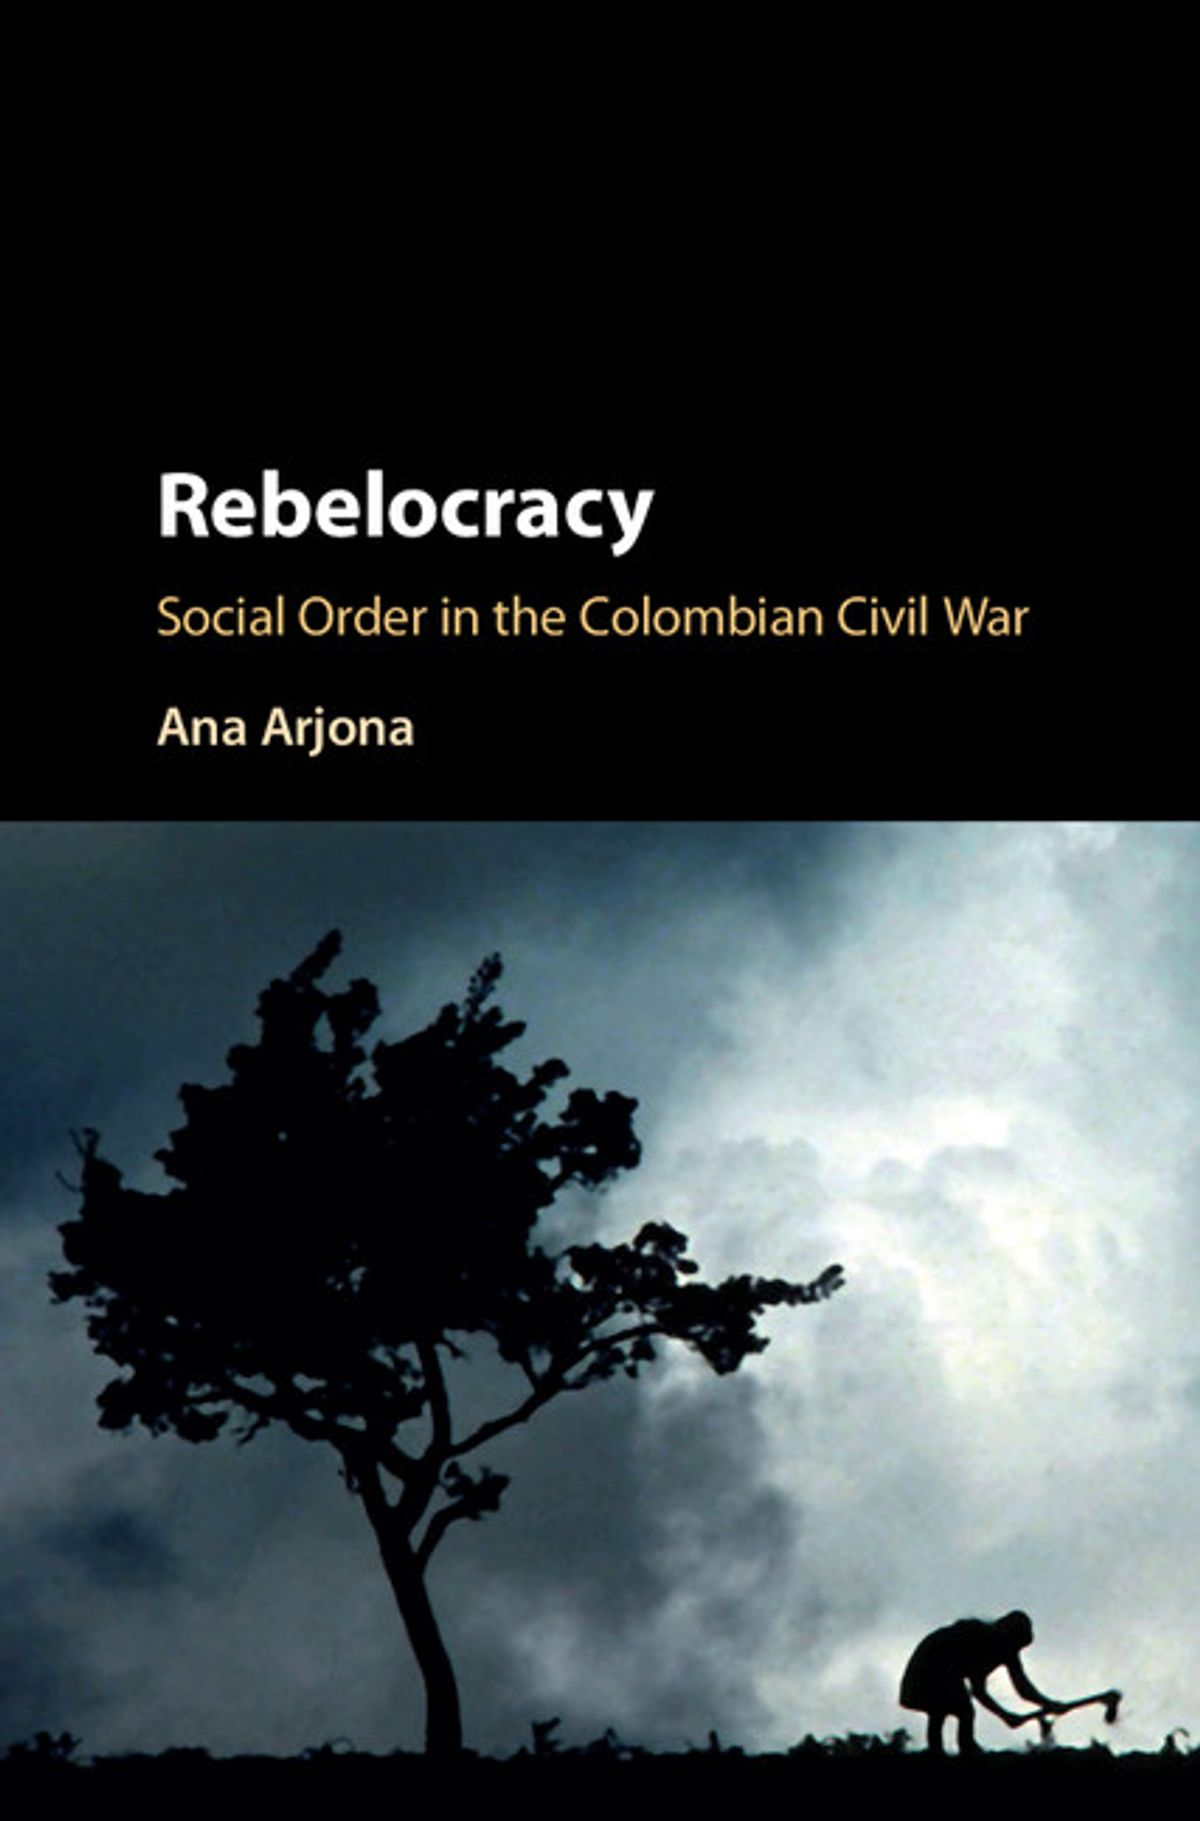
\includegraphics[width = 0.85\textwidth]{img/arjona_rebelocracy}\\
%   {\small Ana Arjona (2017)}
% \end{minipage}

\end{frame}
% ----------------------------------------------------

% ----------------------------------------------------
\begin{frame}
\frametitle{Understanding rebel governance}
\centering

% \begin{minipage}{0.7\textwidth}\centering
  \begin{itemize}[<+->]
    \item[1.] If they have \textbf{long-term expectations} (because of territorial competition, peace agreements, etc), rebels develop more comprehensive governance. Otherwise, there will be disorder
    \item[2.] Rebels prefer \textit{rebelocracy} (replacing and controling all local social institutions), but this is not always possible
    \item[3.] This choice depends on the \textbf{expectation of civilian resistance}, which is shaped by preexisting institutions
    \item[4.] Areas where civilians retain control, rebels establish \textit{aliocracy}: a form of indirect rule, controlling only the basics of security and taxation
  \end{itemize}
% \end{minipage}\hfill
% \begin{minipage}{0.29\textwidth}\centering
%   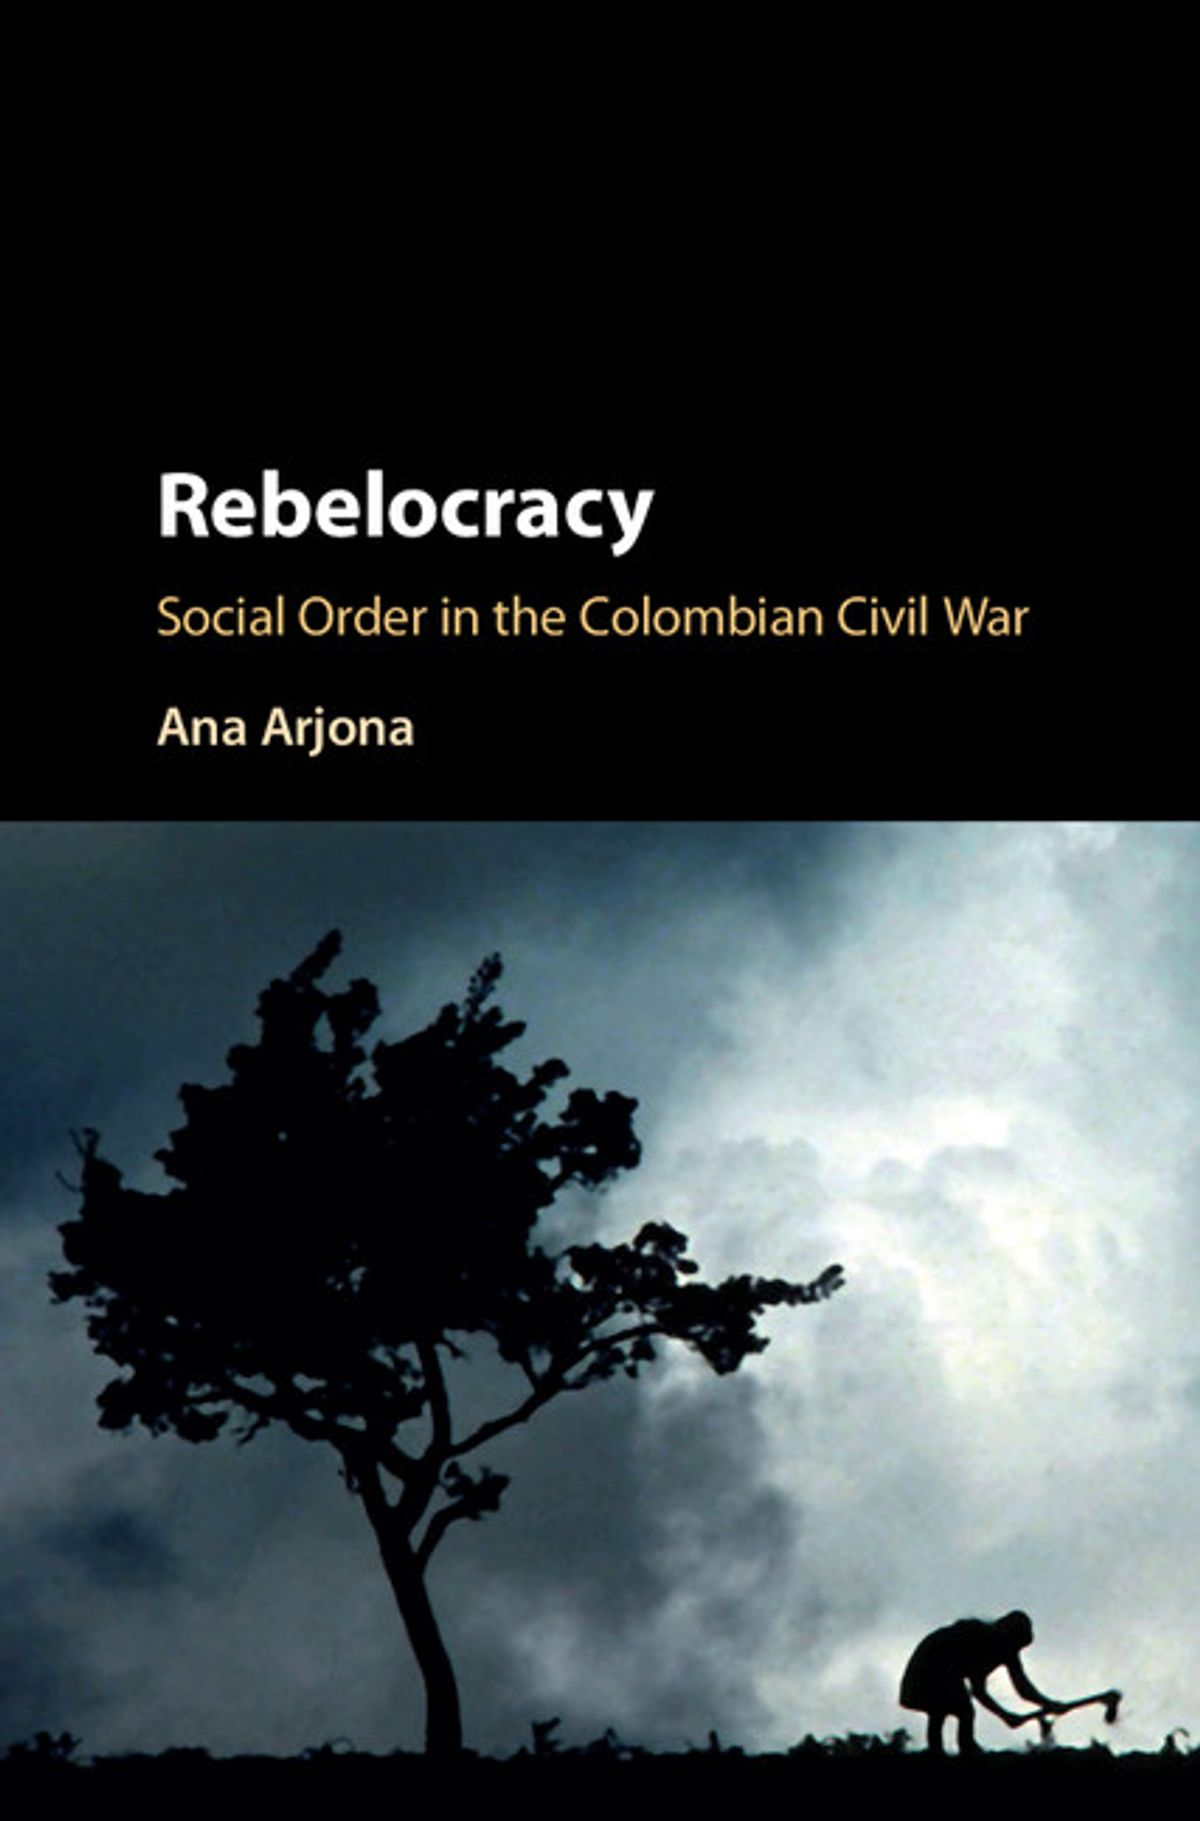
\includegraphics[width = 0.85\textwidth]{img/arjona_rebelocracy}\\
%   {\small Ana Arjona (2017)}
% \end{minipage}

% Arjona explains the variation in rebelocracy, aliocracy and disorder across time and space through the combination of armed groups’ time horizon and the quality of preexisting local institutions. Most rebels care about future outcomes and will seek to regulate private and public life broadly to induce civilian cooperation in areas where they have an ongoing presence. Particularly, they will establish mechanisms to adjudicate disputes, such as courts, as the administration of justice helps ‘armed groups centralize power and build an aura of legitimacy’ (56). Where preexisting institutions shape the capacity for civilians to collectively resist rebel rule and maintain control over civilian affairs, rebels will limit their influence and focus on basic elements of rule: that is, security and taxation. Under certain conditions, when rebels face internal indiscipline, external competition over territory or macro-changes in the war, such as peace negotiations, their focus on short-term goals will lead to disorder, or the absence of social contract in the communities.

\end{frame}
% ----------------------------------------------------

% ----------------------------------------------------
\begin{frame}
\frametitle{Civilian influence and resistance}
\centering

\begin{itemize}
  \item<1-> In brief, it works like a state-building process
  \item<2-> Some degree of opposition is always present, as in any political order
  \item<3-> Full resistance emerges when rebels try to fully replace existing social institutions that are valued locally
  \item<4-> In some cases, local organizations are able to challenge the monopoly of violence of rebels (self-defense etc) or influence local financing and taxation institutions
  \item<5-> Alliance formation (rebels, social sectors/orgs)
\end{itemize}

\end{frame}
% ----------------------------------------------------

% ----------------------------------------------------
\begin{frame}
\frametitle{Beyond governance}
\centering

\begin{minipage}{.59\textwidth}\centering
\begin{itemize}
  \item<1-> Different experiences remembered by recruits for the Salvadorian army vs the FMLN
  \begin{itemize}
    \item Army: forced recruitment, beatings, humiliations...
    \item Rebels: hard training but no abuse, deep political instruction...
  \end{itemize}
  \item<2-> `Internal institutions':
  \begin{itemize}
    \item recruitment
    \item military training
    \item political education
    \item disciplinary measures
  \end{itemize}
  \item<3-> Does it matter?
\end{itemize}
\end{minipage}\hfill
\begin{minipage}{.39\textwidth}\centering
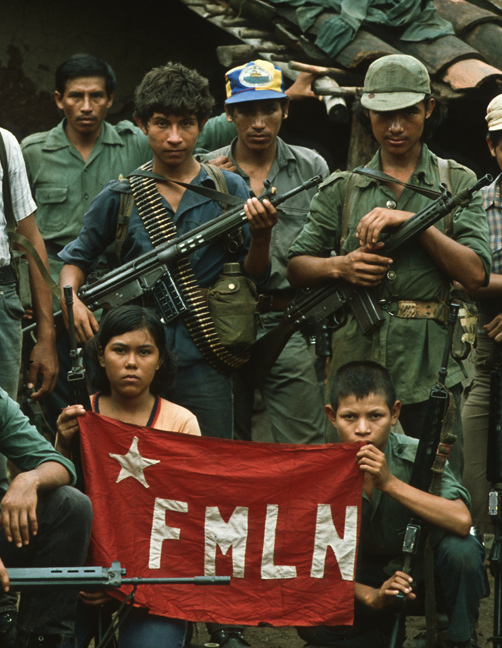
\includegraphics[width = \textwidth]{img/fnml_vert}
\end{minipage}

\end{frame}
% ----------------------------------------------------

% ----------------------------------------------------
\begin{frame}
\frametitle{Beyond governance: killing civilians}
\centering

\begin{minipage}{0.49\textwidth}\centering
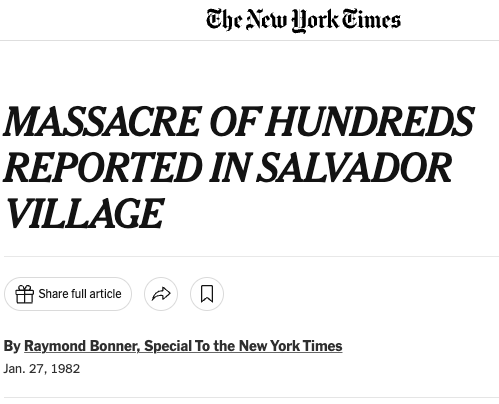
\includegraphics[width = \textwidth]{img/mozote_nyt1}
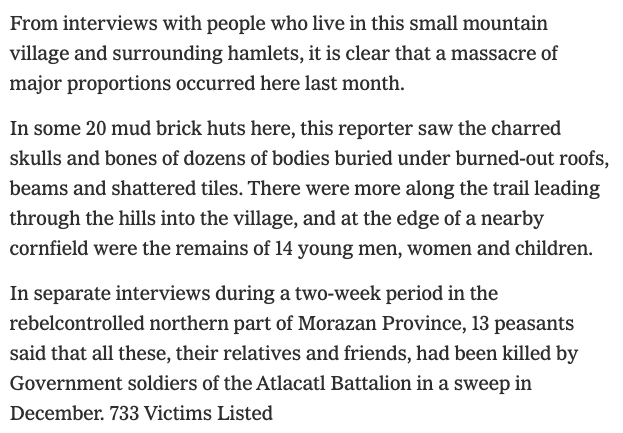
\includegraphics[width = \textwidth]{img/mozote_nyt2}
\end{minipage}\hfill
\begin{minipage}{0.49\textwidth}\centering
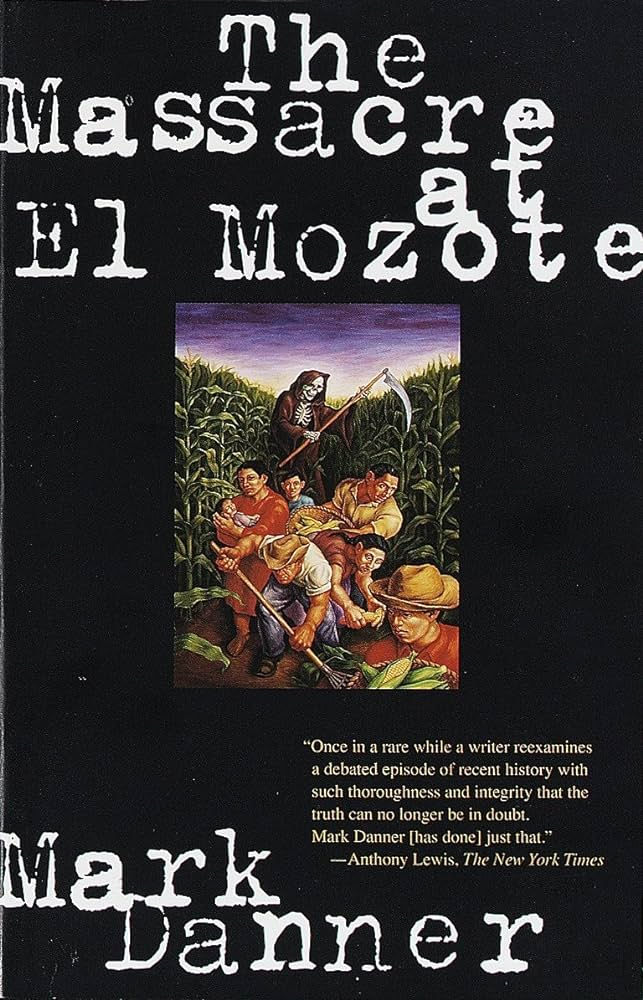
\includegraphics[width = 0.7\textwidth]{img/mozote_book}\\
Dec 1981, almost 1,000 civilians killed, many children \& women
\end{minipage}

\end{frame}
% ----------------------------------------------------

% ----------------------------------------------------
\begin{frame}
\frametitle{Beyond governance: killing civilians}
\centering

\begin{minipage}{.64\textwidth}\centering
\begin{itemize}
  \item<1-> Compare FMLN to Peru's Shinning Path
  \item<2-> The Commander's Dilemma: to win a war, you need to train and arm violent soldiers, but you also need to \textit{control} how and when violence is employed
  \item<2-> When do we observe \BGyellow{restraint}? When commanders create institutions to discipline soldiers and socialize them politically
\end{itemize}
\end{minipage}\hfill
\begin{minipage}{.34\textwidth}\centering
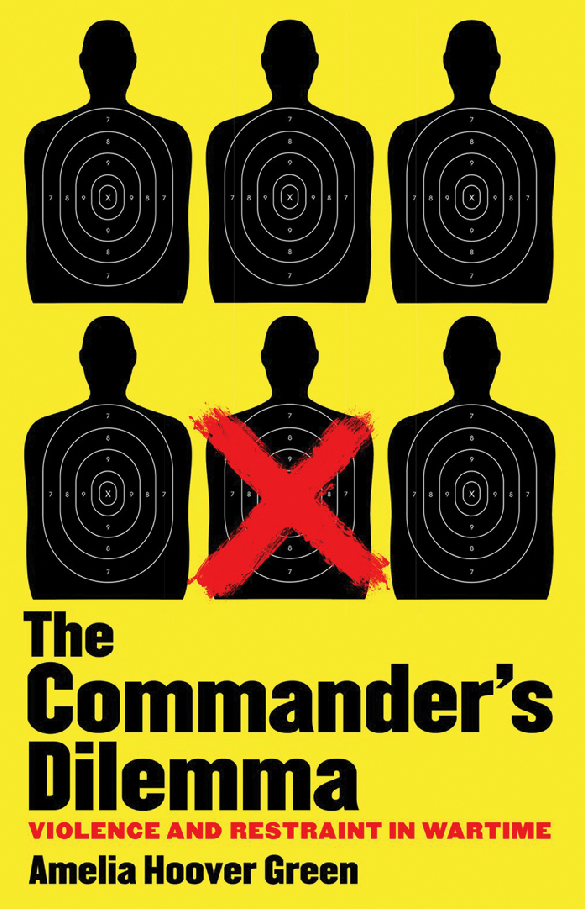
\includegraphics[width = 0.8\textwidth]{img/hoover_green}\\Hoover Green (2018)
\end{minipage}

\end{frame}
% ----------------------------------------------------

% ----------------------------------------------------
\begin{frame}<1-2>[label=rape]
\frametitle{Beyond governance: sexual violence}
\centering

\begin{itemize}
  \item<1-> What explains wartime sexual violence?
  \item[]
  \item[1.]<2-> Rape as \textit{collateral} violence, opportunistic \& private reasons
  \item[2.]<3-> Rape as \textit{strategic} violence
  \begin{itemize}
    \item Sexual violence offers organizational advantages related to warfare
  \end{itemize}
  \item<4-> Rape as \textbf{practice}
  \begin{itemize}
    \item Socialization, organizational aspects, absence of restraint, etc
  \end{itemize}
\end{itemize}

\end{frame}
% ----------------------------------------------------

% ----------------------------------------------------
\begin{frame}
\frametitle{Beyond governance: sexual violence}
\centering

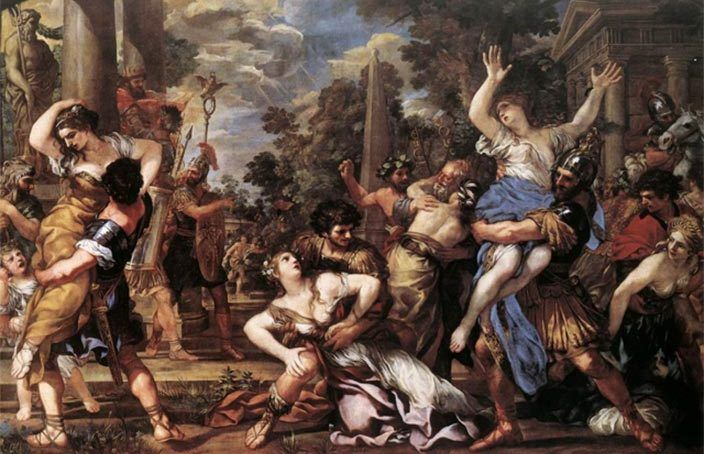
\includegraphics[width = 0.9\textwidth]{img/rape_history}

\end{frame}
% ----------------------------------------------------

% ----------------------------------------------------
\againframe<3>{rape}
% ----------------------------------------------------

% ----------------------------------------------------
\begin{frame}
\frametitle{Beyond governance: sexual violence}
\centering

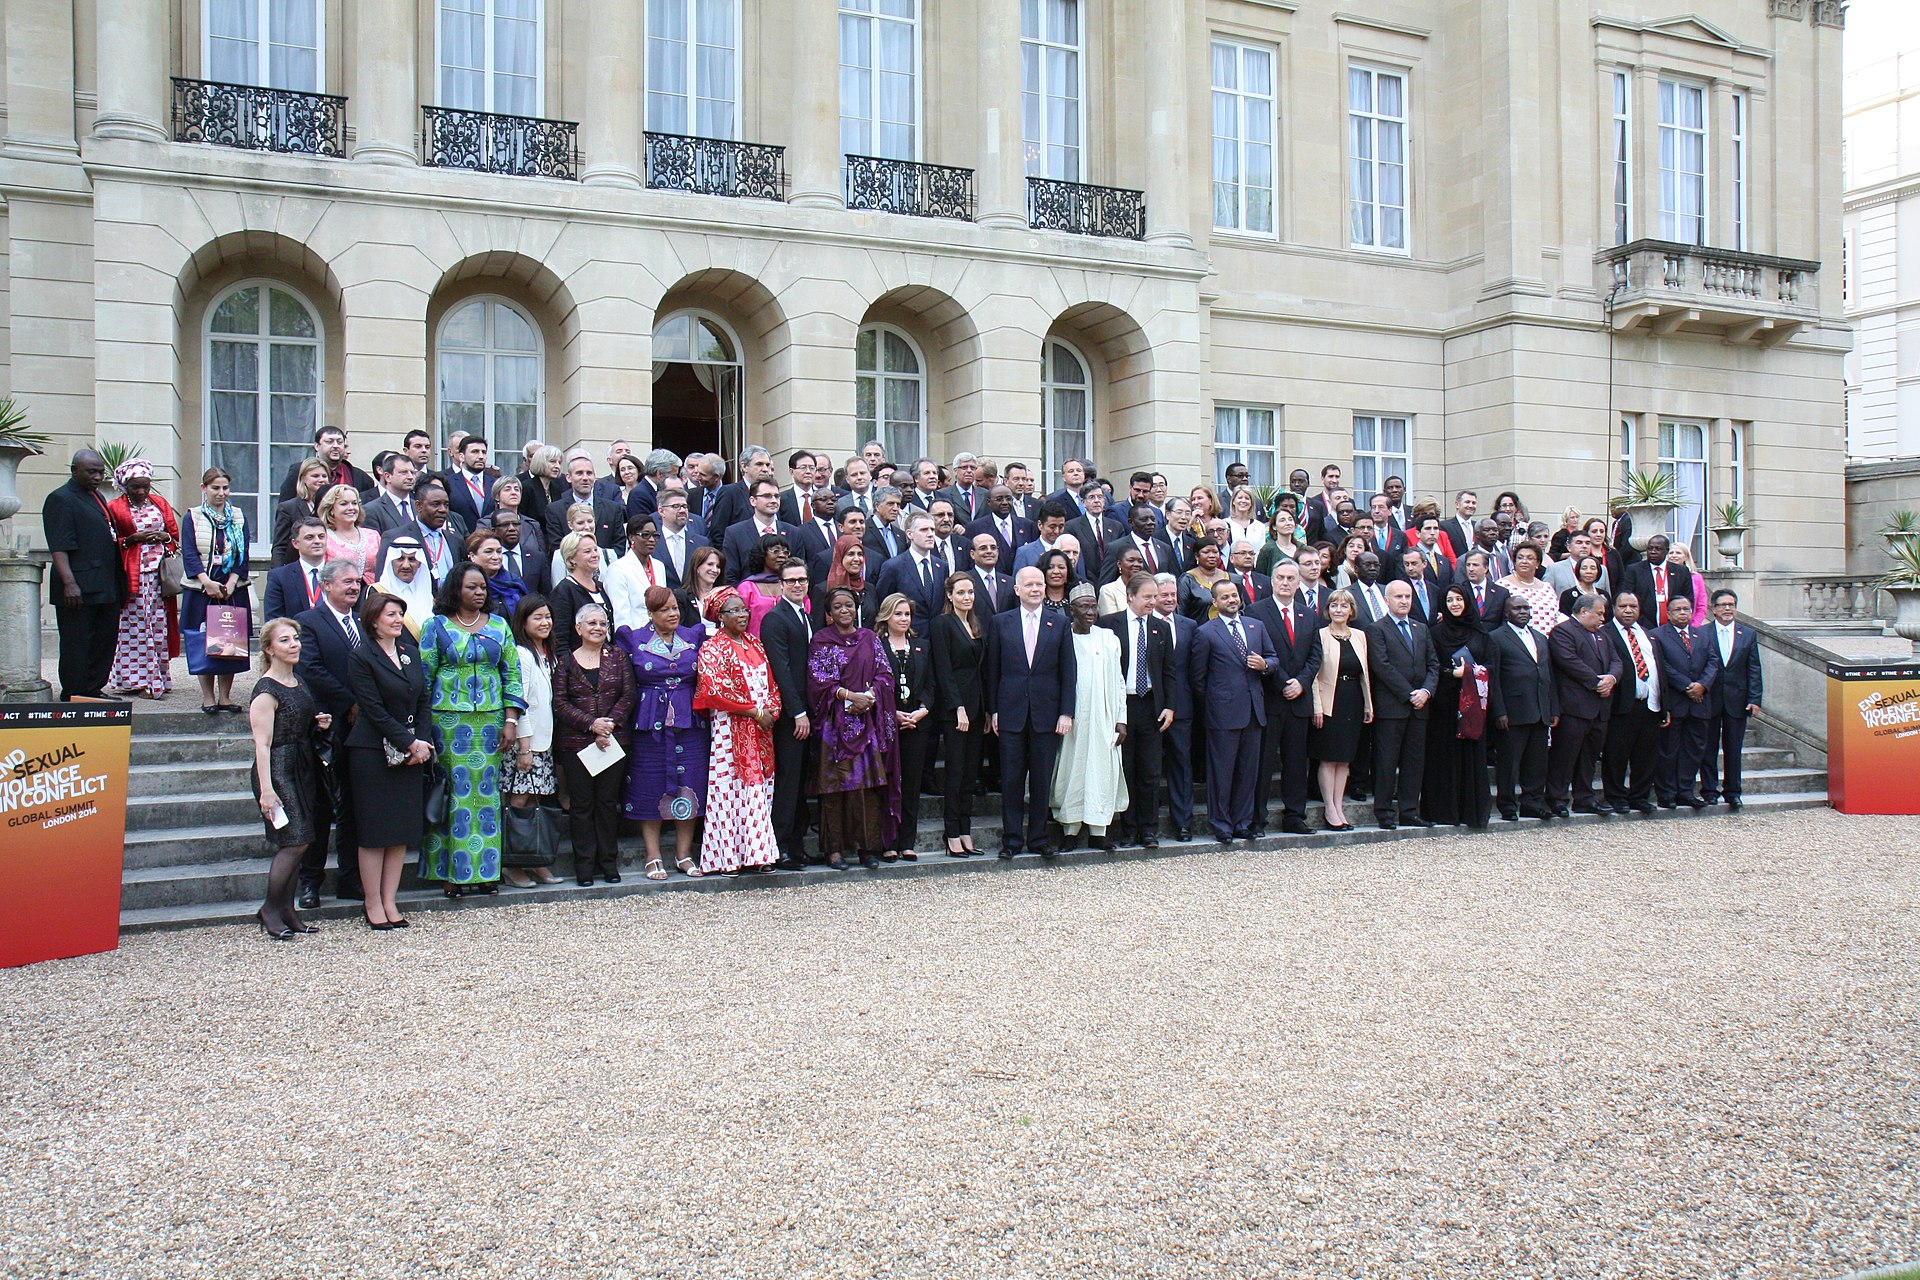
\includegraphics[width = 0.8\textwidth]{img/global_summit_rape}

Global Summit to End Sexual Violence in Conflict, 2014

\end{frame}
% ----------------------------------------------------

% ----------------------------------------------------
\againframe<4>{rape}
% ----------------------------------------------------

% ----------------------------------------------------
\begin{frame}
\frametitle{Beyond governance: sexual violence}
\centering

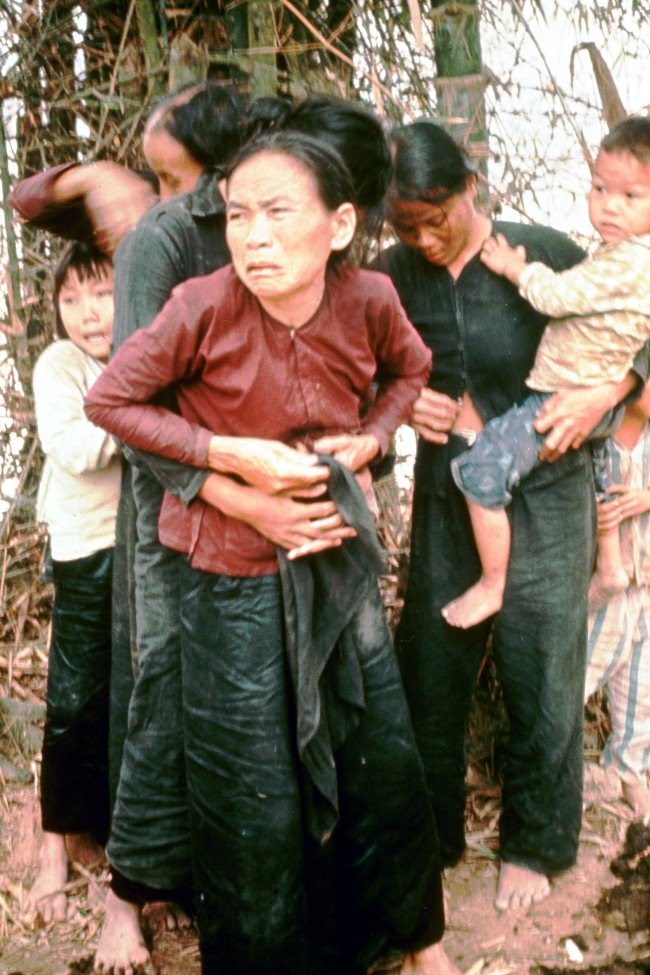
\includegraphics[width = 0.4\textwidth]{img/my_lai}

US troops in Vietnam, My Lai massacre (1968)

\end{frame}
% ----------------------------------------------------

% % ----------------------------------------------------
% \begin{frame}
% \frametitle{Beyond civil wars: gangs}
% \centering
%
% 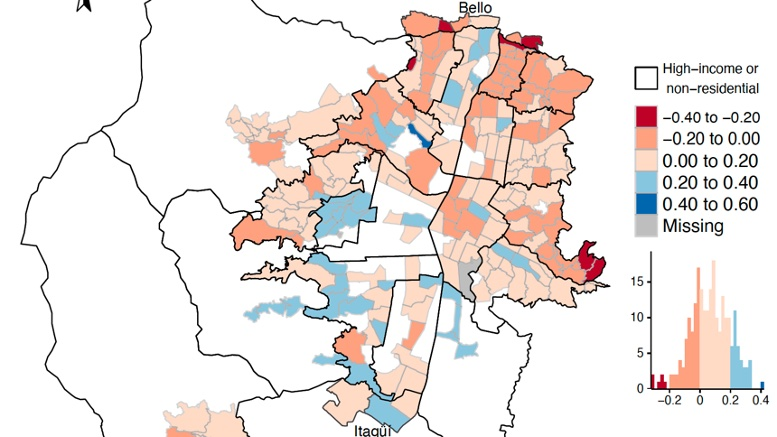
\includegraphics[width = 0.85\textwidth]{img/combo_governance_medelling}
%
% Service provision by local gangs in Medellin (red means that the role of combo $>$ role of state)
%
% \vspace{15pt}
%
% {\footnotesize \textit{Source:} Chris Blattman et al)}
%
% \end{frame}
% % ----------------------------------------------------

% ----------------------------------------------------
\begin{frame}
\frametitle{Beyond civil wars: gangs}
\centering

% CHRIS BLATTMAN:
% https://twitter.com/cblatts/status/1311474471874760704

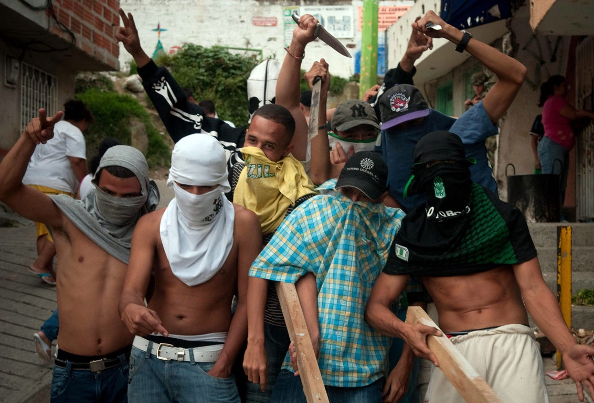
\includegraphics[width = 0.8\textwidth]{img/combo}

\vspace{15pt}

`Combo' members in Colombia

\end{frame}
% ----------------------------------------------------

% % ----------------------------------------------------
% \begin{frame}
% \frametitle{Beyond civil wars: gangs}
% \centering
%
% 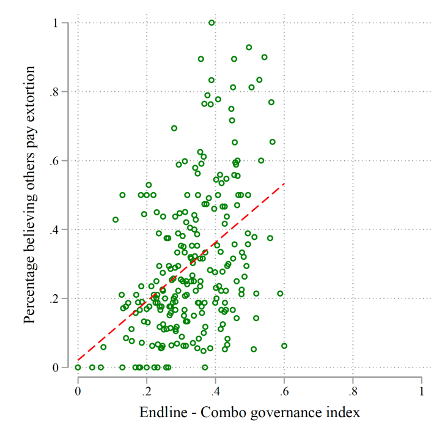
\includegraphics[width = 0.5\textwidth]{img/combo_gov_index_taxation}
%
% Gangs governance: it will be related to taxes/extortion, but it's also a choice
%
% \vspace{15pt}
%
%
% \end{frame}
% % ----------------------------------------------------

% % ----------------------------------------------------
% \begin{frame}
% \frametitle{Beyond civil wars: gangs}
% \centering
%
% \begin{itemize}
%   \item Where should we see combos more likely to engage in governance?
% \end{itemize}
%
% \vspace{15pt}
%
%
% \end{frame}
% % ----------------------------------------------------

% % ----------------------------------------------------
% \begin{frame}
% \frametitle{Beyond civil wars: gangs}
% \centering
%
% 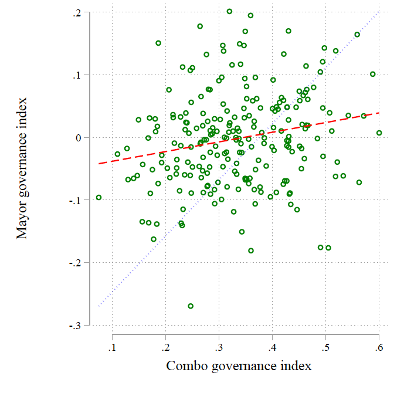
\includegraphics[width = 0.5\textwidth]{img/combo_mayor_gov_index}
%
% Gangs governance and local government, they overlap
%
% \vspace{15pt}
%
% \end{frame}
% % ----------------------------------------------------

\end{document}
